\documentclass[a4paper,10pt]{report}

\usepackage[utf8]{inputenc}
\usepackage[T1]{fontenc}
\usepackage[UKenglish]{babel}
\usepackage{titlesec}
\usepackage[backend=biber, style=numeric, sorting=nty, defernumbers=true]{biblatex}
\addbibresource{sources.bib}

\usepackage[top=20mm, bottom=20mm, left=20mm, right=20mm]{geometry} % définit les marges
\usepackage{array} % permet l'alignement vertical dans les tableaux
\usepackage{setspace} % permet de régler l'interligne
\onehalfspacing % définit l'interligne 1,5 par défaut

%\usepackage{fourier} % modifie la police par défaut
\usepackage[osf]{newpxtext} % osf for text, not math
\usepackage{cabin} % sans serif
\usepackage[varqu,varl]{inconsolata} % sans serif typewriter
\usepackage[bigdelims,vvarbb]{newpxmath} % bb from STIX
\usepackage[cal=boondoxo]{mathalfa} % mathcal
\usepackage{mathtools}

\usepackage{xcolor}
\definecolor{taucolor}{rgb}{0.0,0.2,0.4} 
\usepackage[colorlinks=true,allcolors=taucolor]{hyperref}
\usepackage{cleveref}
\usepackage{bookmark}

\newcommand{\figlabel}{{Fig.}}
\newcommand{\figslabel}{{Figs.}}
\newcommand{\tablabel}{{Table}}
\newcommand{\captionlabelcode}{{Code}}   
\newcommand{\eqlabel}{{Equation}}
\newcommand{\figref}[1]{\hyperref[#1]{\figlabel~\ref*{#1}}}
\newcommand{\figsref}[1]{\hyperref[#1]{\figslabel~\ref*{#1}}}
\newcommand{\tabref}[1]{\hyperref[#1]{\tablabel~\ref*{#1}}}
\newcommand{\coderef}[1]{\hyperref[#1]{\captionlabelcode~\ref*{#1}}}
\newcommand{\equref}[1]{\hyperref[#1]{\eqlabel~\ref*{#1}}}

\setlength{\tabcolsep}{18pt}
\renewcommand{\arraystretch}{1.5}
\setlength{\parindent}{0pt}

\usepackage{graphicx}
\usepackage{here}
\graphicspath{{figures/}{./}} 
\usepackage{subcaption}

\title{}
\author{Arthur Thomas}
\date{June 2027}

\begin{document}

\begin{titlepage} 
\singlespacing 

\begin{center} 
\huge{\textsc{Université Libre de Bruxelles}}\\
\vspace{.5cm}
\LARGE{Faculté des Sciences}\\
\vspace{.3cm}
\Large{Département de Physique}
\end{center}

\vspace{1cm} 

\begin{center}
  
\includegraphics[width=\linewidth/4]{ULBlogo.jpg}
\end{center}

\vspace{1cm}

\begin{center}
\Huge{Proton structure !}\\
\vspace{.5cm}
\LARGE{Generating the transverse distributions from first principles} 
\end{center}

\vfill

\begin{tabular}{b{5.5cm}b{7.5cm}} 
\large{Arthur \textsc{Thomas}} & Mémoire présenté sous la direction de Laurent \textsc{Favart} et Andris \textsc{Potrebko} en vue de 
l'obtention du titre de Master en Sciences Physiques\\ 
\end{tabular}

\vfill

\begin{center}
Année académique 2026--2027
\end{center}

\end{titlepage}

\tableofcontents

\newpage

\section*{Résumé}
\addcontentsline{toc}{section}{Résumé}
\section*{Abstract}
\addcontentsline{toc}{section}{Abstract}

\newpage

\chapter*{Introduction}
\addcontentsline{toc}{chapter}{Introduction}%\stepcounter{chapter}
Idées principales, contexte, intérêt, déroulé\\

Citations temporaires pour que tout apparaisse dans la bibliographie : 
\cite{Hautmann_2018}, \cite{hj_lect}, \cite{Lelek}, \cite{cours1}, \cite{Ellis_Stirling_Webber_1996}

\newpage

\chapter{À déterminer+}
1-2 chapitres sur le background théorique (DGLAP, parton branching, plus de détails sur le contexte?)

\newpage

\chapter{A simplified parton evolution}

In this section, we will show how to numerically compute PDFs and TMDs with a parton 
branching method, with a very simplified framework, taken from the exercises adjoining \cite{hj_lect}. 
Even if this implementation is far less sophisticated than the one this thesis is focused on, it 
already holds many of its key points, and will allow us, by fiddling with its parameters, to 
investigate its behavior and reveal points of interest to keep in mind for the full implementation. \\
\textit{\textbf{Note : }This is the reason why completing the exercises from \cite{hj_lect} was the first step of 
my assignment. The parton evolution presented here is a slight variation of exercise 3 of these 
lectures. I used \cite{hj_lect} and \cite{Lelek} as a guide to complete it.}\\
We won't refer to the literature here, mainly because 
this toy framework will most certainly not produce accurate results with respect to experimental data. 
Still, it shouldn't be too far off, and we might have considered using some established results in 
order to have a qualitative idea of what to expect. Nevertheless, the following plots will be discussed here with 
no \textit{a priori}, as a first exposure to the parton branching method. The commentaries in this chapter 
are more destined to help build a picture and gather ideas than to describe rigorously quantitative 
properties.

    \section{Implementation}

    We want to evolve a starting gluon density $f(x, \mu_0^2) = 3(1-x)^5/x$ from scale 
    $\mu_0^2 = 1\,\text{GeV}^2$ to scale $\mu_f^2=10\,000\,\text{GeV}^2$. We will also generate 
    their transverse momentum $k_t$ during the evolution, and assuming a starting distribution 
    with zero mean and $\sigma = 0.7\,\text{GeV}$. We will use the splitting function 

    \begin{equation}
    P_{gg}(z) = 6\left(\frac{1}{z} + \frac{1}{1-z}\right)
    \label{eq:simp_pgg}
    \end{equation} 
    
    with cut-offs $z_{min} = \epsilon,\, z_{max} = 1 - \epsilon$ 
    with $\epsilon = 0.1$. As a last simplification, we will take the strong coupling to be 
    constant : $\alpha_s = 0.1$. \\ 
    We will also redo the same exercise, with a quark-quark splitting 
    
    \begin{equation}
    P_{qq}(z) = \frac{4}{3}\frac{1+z^2}{1-z}
    \label{eq:simp_pqq}
    \end{equation}
    
    and assuming the same starting distribution (which could pass as an approximation of a sea quark 
    density, but not a valence quark density).\\

    In order to evaluate the density at the final scale, $f(x, \mu_f^2)$, we will generate $1\,000\,000$
    events from the starting density and evolve them by simulating their possible branching 
    according to the known probability densities. The evolved events will then be distributed 
    following $f(x, \mu_f^2)$. During the evolution of each event, we will also generate the 
    $k_t$ of the emitted gluon, and compute the change of $k_t$ of the emitter, to obtain a 
    $k_t$ distribution at the final scale. \\ 

    For each event, we must perform the following steps : 

    \begin{enumerate}
        \item \textbf{Generate the starting momentum fraction $x_0$ and transverse momentum $k_{t,0}$ :}
        
              Here, we generate $x_0$ with the importance sampling method, using the approximate 
              function \\$g(x) = \frac{1}{x\,\log(x_{max}/x_{min})}$, with $x_{min} = 0.000\,01$ and $x_{max} = 1$.\\
              Then, drawing a uniform random number $R_{x_0} \in [0,1]$, we get $x_0$ and its weight $w_{x_0}$ as 

              \begin{align}
              \setlength\fboxsep{1em}
              \Aboxed{x_0 &= x_{min}\,\left(\frac{x_{max}}{x_{min}}\right)^{R_{x_0}}} \\
              \setlength\fboxsep{1em}
              \Aboxed{w_{x_0} &= 3\,(1-x_0)^5\,\log(x_{min}/x_{max})}  \label{eq:simp_wx0}   
              \end{align}
              
              We generate $k_{t,0}$ using the central limit theorem, by summing 12 uniform random numbers 
              $R_i \in [0,1]$, with then

              \begin{equation}
                \setlength\fboxsep{1em}
                \boxed{k_{t,0} = 0.7\,\left(\sum_{i=1}^{12}R_i -6\right)}
              \end{equation}

              These will indeed distribute following a Gaussian distribution of mean 0 and standard 
              deviation 0.7. We also need the two components $k_{x,0}$ and $k_{y,0}$ for later use, 
              so we draw a uniformly distributed azimuthal angle $\phi \in [0, 2\pi]$ to initialise 
              them at $k_{x,0} = k_{t,0}\cos(\phi)\,,\,k_{y,0} = k_{t,0}\sin(\phi)$.\\

        \item \textbf{Generate the next branching scale $\mu_i^2$}
        
              We generate the next scale $\mu_i^2$ with respect to the Sudakov form factor

              \begin{equation}
              \Delta_S(\mu_{i-1}^2, \mu_i^2) = \exp\left(-\int_{\mu_{i-1}^2}^{\mu_i^2}\frac{d\mu^2}{\mu^2}\int_{z_{min}}^{z_{max}}dz\frac{\alpha_s}{2\pi}P_{gg}(z)\right)
              \end{equation}

              by drawing a uniformly distributed random number $R_{\mu_i^2} \in [0,1]$ and inverting 
              the relation $R_{\mu_i^2} = \Delta_S(\mu_{i-1}^2, \mu_i^2)$. In our case, it is easy 
              since the only scale dependence is in the $1/\mu^2$ term, as we are approximating 
              $\alpha_s$ to be constant. Thus we have 

              \begin{align}
                \ln(R_{\mu_i^2}) &= -\int_{\mu_{i-1}^2}^{\mu_i^2}\frac{d\mu^2}{\mu^2}\int_{z_{min}}^{z_{max}}dz\frac{\alpha_s}{2\pi}
                6\left(\frac{1}{z} + \frac{1}{1-z}\right) \nonumber \\
                \Leftrightarrow \quad 
                \ln(R_{\mu_i^2}) &= -\frac{\alpha_s}{2\pi}\ln\left(\frac{\mu_i^2}{\mu_{i-1}^2}\right)
                6\left[\ln\left(\frac{z_{max}}{1-z_{max}}\right) - \ln\left(\frac{z_{min}}{1-z_{min}}\right)\right] \nonumber \\
                \Leftrightarrow \quad
                \ln\left(\frac{\mu_i^2}{\mu_{i-1}^2}\right) &= 
                -\frac{\pi}{3\alpha_s}\ln\left(\frac{z_{max}(1-z_{min})}{(1-z_{max})z_{min}}\right)^{-1}\ln(R_{\mu_i^2}) \nonumber \\
                \Leftrightarrow \quad
                \setlength\fboxsep{1em}
                \Aboxed{\mu_i^2 &= \mu_{i-1}^2\,R_{\mu_i^2}^{-\frac{\pi}{3\alpha_s}\ln\left(\frac{z_{max}(1-z_{min})}{(1-z_{max})z_{min}}\right)^{-1}}}
                \label{eq:simp_scalegen}
              \end{align}

              With the quark-quark splitting function $P_{qq}(z)$ from \equref{eq:simp_pqq}, the exponent becomes 

              \begin{equation}
              -\frac{3\pi}{2\alpha_s}\left(\frac{z_{min}^2-z_{max}^2}{2}+(z_{min}-z_{max})+2\ln\left(\frac{1-z_{min}}{1-z_{max}}\right)\right)^{-1}
              \end{equation}

              We then compare the new scale with the final scale : if $\mu_i^2 > \mu_f^2$, this 
              means that no branching occurred up to the final scale, and we keep the last 
              $x_i$ and $k_{t,i}$ generated. If not, then a branching occurred at this scale, 
              and we carry on with the following steps to generate its effect.\\

        \item \textbf{Generate the splitting variable $z_i$ and the new $k_{t,i}$}
        
              The splitting variable is generated in a similar way, using the normalised integrated
              splitting function as the cumulative function. So, with a uniformly generated random 
              number $R_{z,i} \in [0,1]$, we have 

              \begin{align}
                R_{z,i} &= \frac{\int_{z_{min}}^{z_i}dz\,P_{gg}(z)}{\int_{z_{min}}^{z_{max}}dz\,P_{gg}(z)} \nonumber \\
                \Leftrightarrow \quad
                R_{z,i} &= \frac{6\left(\ln\left(\frac{z_i}{1-z_i}\right)-\ln\left(\frac{z_{min}}{1-z_{min}}\right)\right)}{6\left(\ln\left(\frac{z_{max}}{1-z_{max}}\right)-\ln\left(\frac{z_{min}}{1-z_{min}}\right)\right)} \nonumber \\
                \text{posing}\quad \Aboxed{A &= R_{z,i}\ln\left(\frac{z_{max}}{1-z_{max}}\right) + (1-R_{z,i})\ln\left(\frac{z_{min}}{1-z_{min}}\right)} \nonumber \\ 
                \Leftrightarrow \quad 
                \frac{z_i}{1-z_i} &= e^A \nonumber \\ 
                \Leftrightarrow \quad 
                \setlength\fboxsep{1em}
                \Aboxed{z_i &= \frac{e^A}{1 + e^A}}
              \end{align}

              For the quark-quark splitting of \equref{eq:simp_pqq}, inverting the relation is more tricky. 
              We prefer to use importance sampling again, using as an approximate function 
              $g(z) = \frac{1}{(1-z)\ln\left(1-z_{min}/1-z_{max}\right)}$ with thus 

              \begin{align}
                z_i &= 1 - (1-z_{min})\left(\frac{1-z_{max}}{1-z_{min}}\right)^{R_{z_i}} \\
                &\text{with weight} \nonumber\\ 
                w_{z_i} &= \frac{4}{3}(1+z_i^2)\ln\left(1-z_{min}/1-z_{max}\right)
              \end{align}

              We can then update the momentum fraction by multiplying the previous one with the new splitting variable : 

              \begin{equation}
                x_i = z_i\, x_{i-1}
              \end{equation}

              In the quark case, we also need to multiply the weight : $w_{x_i} = w_{z_i}\, w_{x_{i-1}}$ while 
              in the gluon case, the weight stays at its initial value from \equref{eq:simp_wx0}.

              We can also generate the new $k_{t,i}$. Actually, we generate the $k_t$ of the emitted 
              particle, then calculate the resulting $k_{t,i}$ of the emitter. The choice of expression
              for the $k_t$ is not set in stone, we have to make a heuristic choice. Here, we will investigate two 
              options : \textit{transverse ordering} and \textit{angular ordering}. The former prescribe 
              
              \begin{equation}
                k_t = \mu_i
                \label{eq:simp_trord}
              \end{equation}

              Where the natural scale for the $k_t$ is then taken to be the current energy scale. The latter uses

              \begin{equation}
                k_t = \mu_i\,(1-z_i)
                \label{eq:simp_angord}
              \end{equation}

              Which rather associate the energy scale with the angle of the momentum of the emitted particle, with 
              respect to the one of the emitter. The discussion on how these are obtained is deferred to the next chapter.
              In the meantime, we will just use them as-is to investigate the resulting distributions.\\
              In the following analysis, we will try angular ordering first, and transverse ordering second. \\

              Generating a uniformly distributed azimuthal angle $\phi \in [0,2\pi]$, we can finally evaluate
              
              \begin{equation}
                \setlength\fboxsep{1em}
                \boxed{k_{x_i} = k_{x_{i-1}}-k_t\cos\phi \quad ;\quad k_{y_i} = k_{y_{i-1}}-k_t\sin\phi
                \quad ; \quad k_{t_i} = \sqrt{k_{x_i}^2 + k_{y_i}^2}}
              \end{equation}

        \item \textbf{Jump back to 2. until the end of the loop}

    \end{enumerate}

    Going through these steps looks like this (with angular ordering for the $k_t$ generation) :

    \begin{figure*}[h]
    \centering
    \begin{subfigure}[b]{0.31\linewidth}
      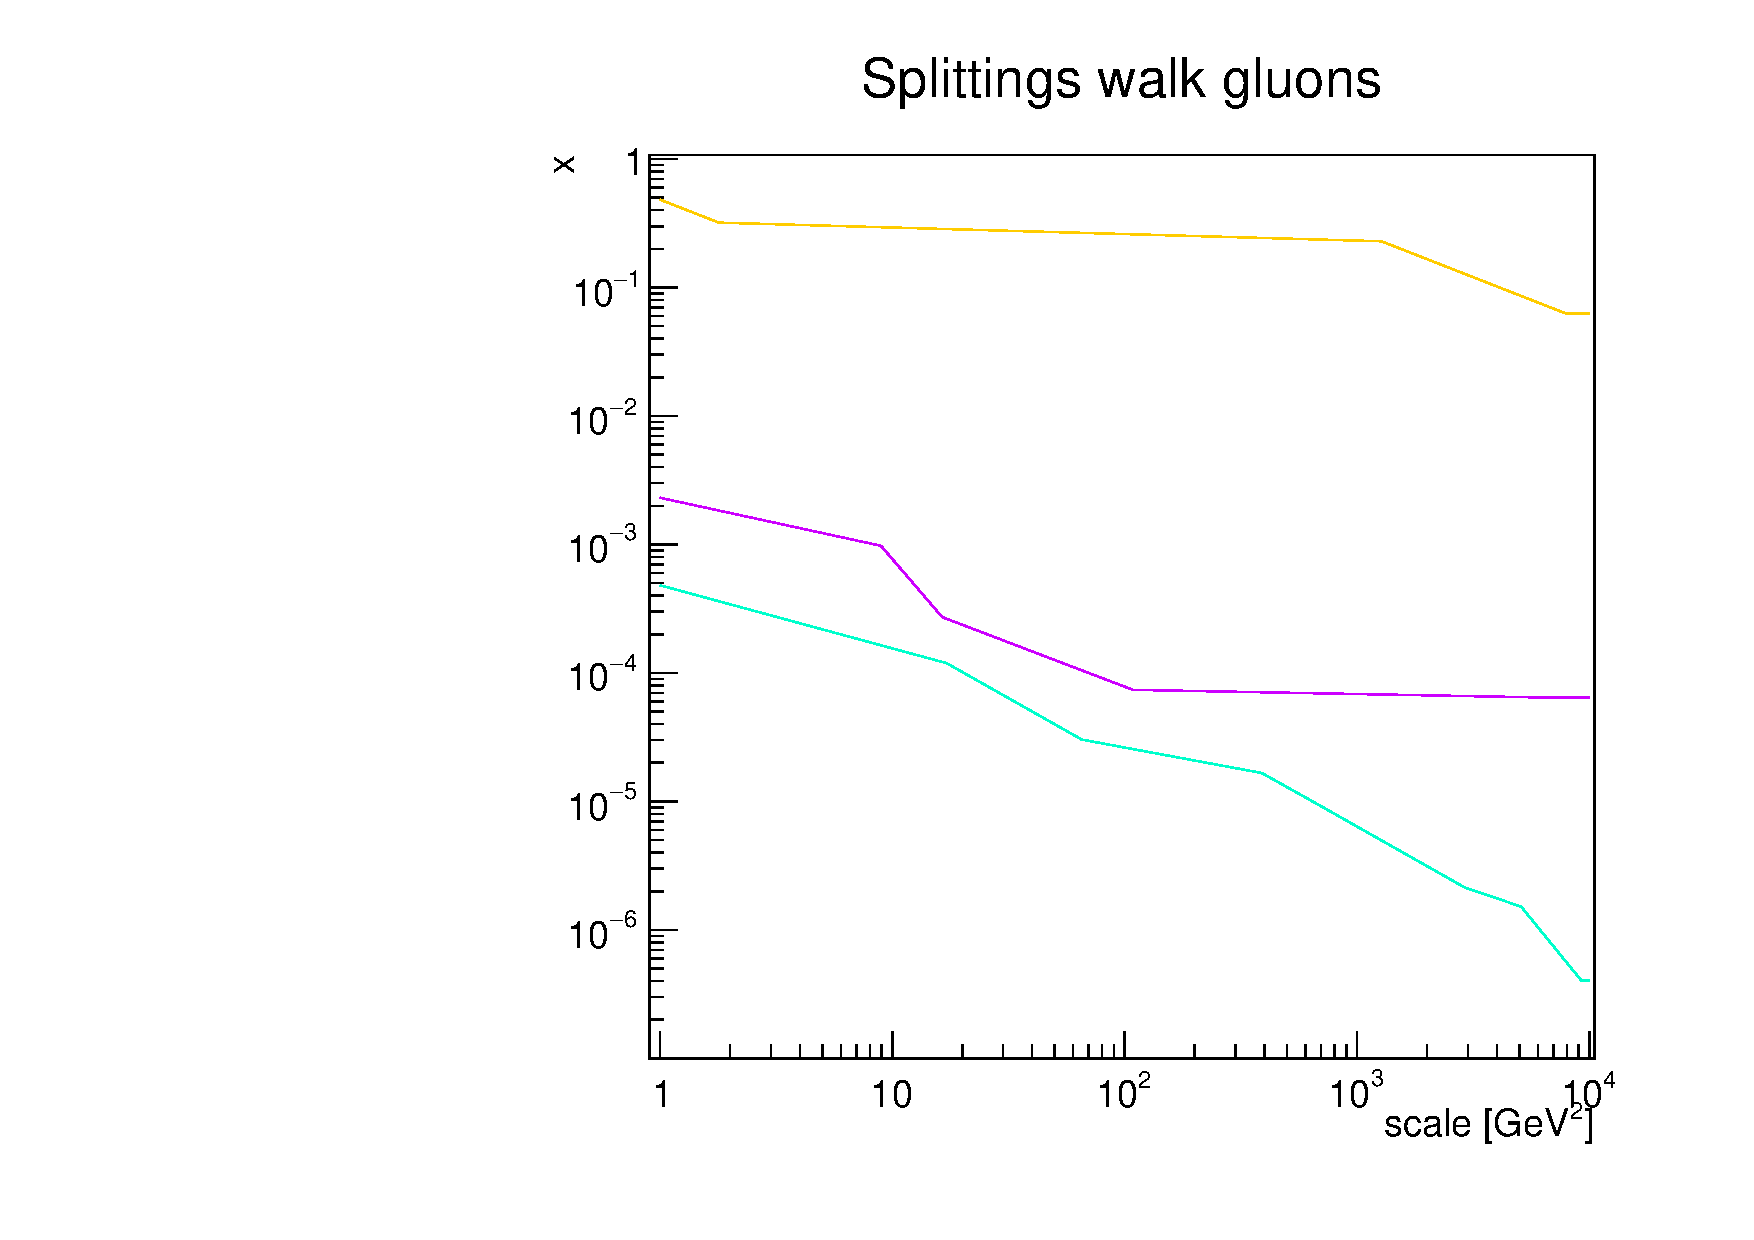
\includegraphics[width=\linewidth]{a-walksz-Pgg.pdf}
			\caption{sample gluon evolution}
			\label{fig:simp_egz1}
    \end{subfigure}
      \hspace{10pt}
    \begin{subfigure}[b]{0.31\linewidth}
      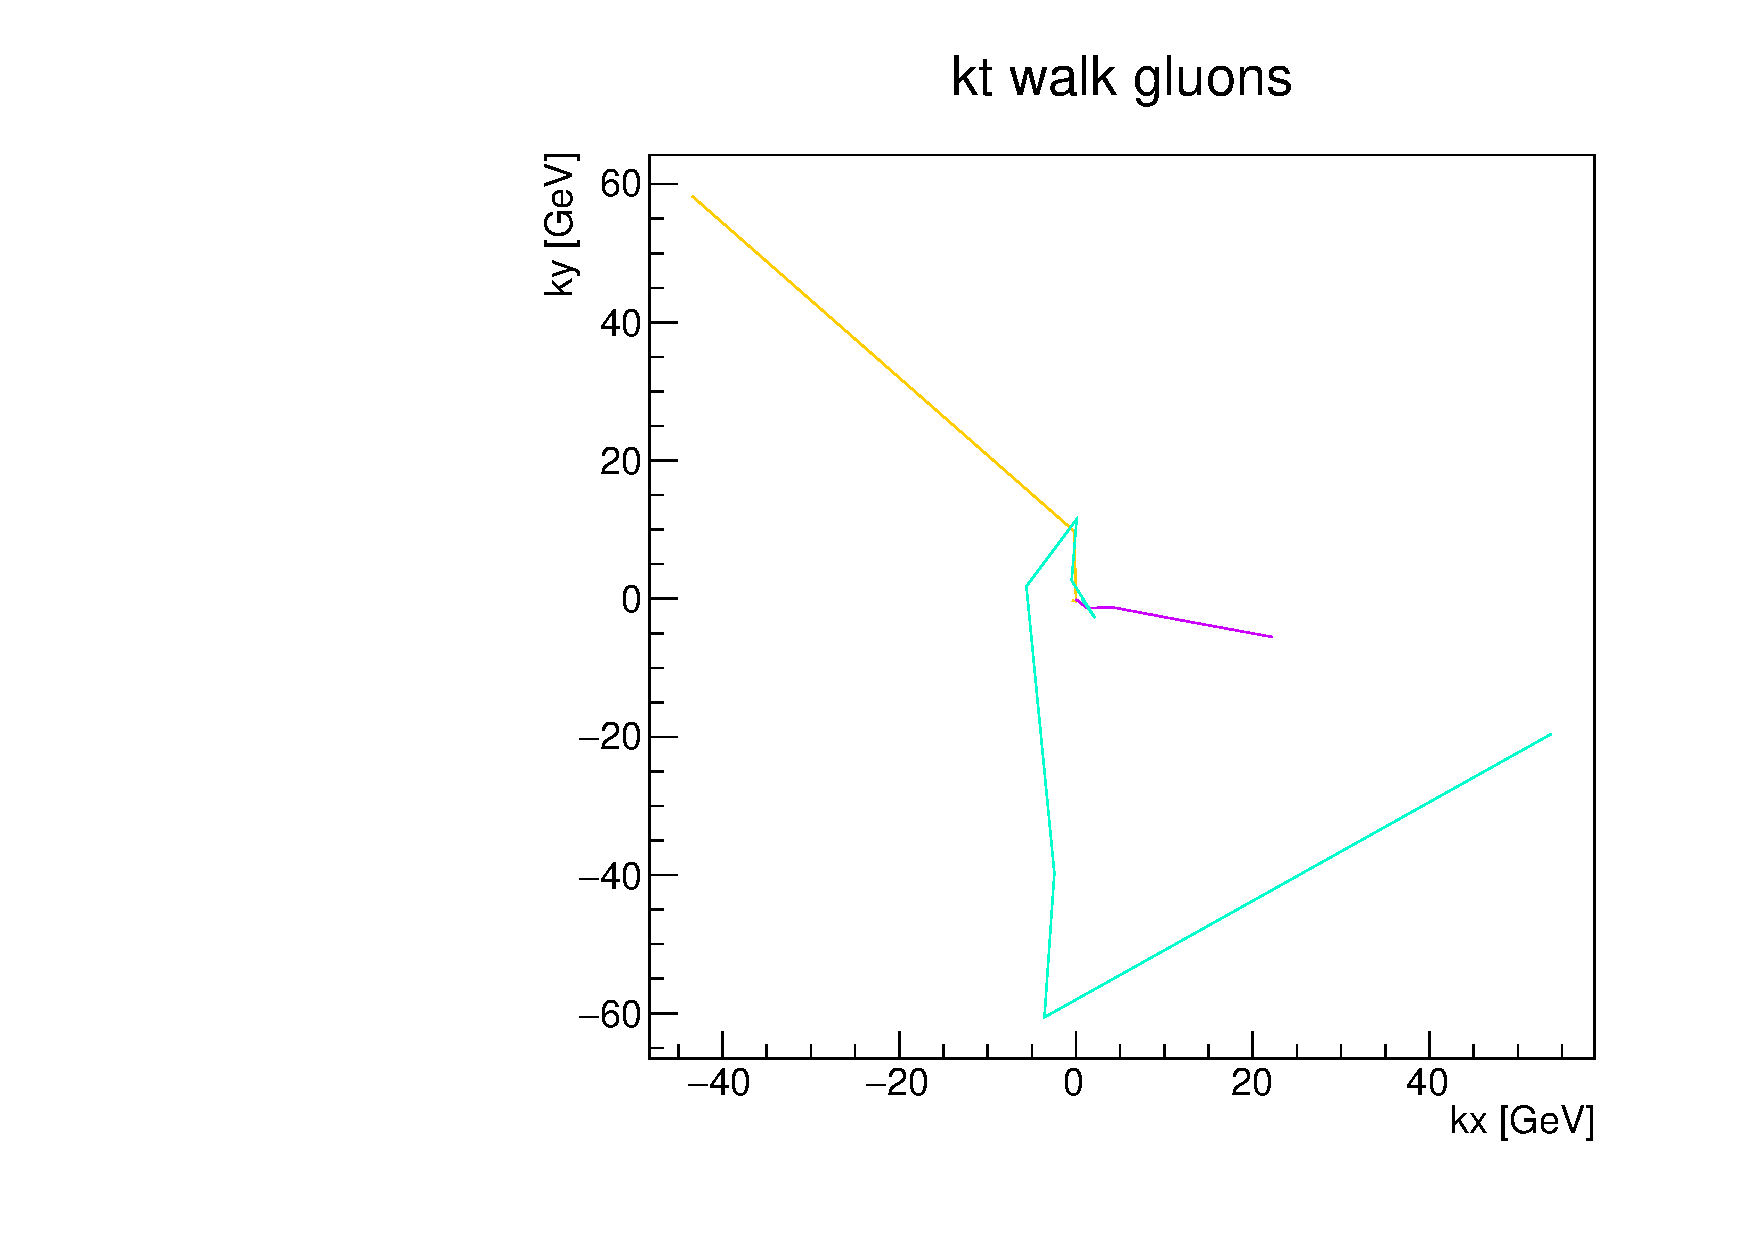
\includegraphics[width=\linewidth]{a-walksktxy-Pgg.pdf}
			\caption{sample gluon $k_t$ generation}
			\label{fig:simp_egkxy1}
    \end{subfigure}
      \hspace{10pt}
    \begin{subfigure}[b]{0.31\linewidth}
      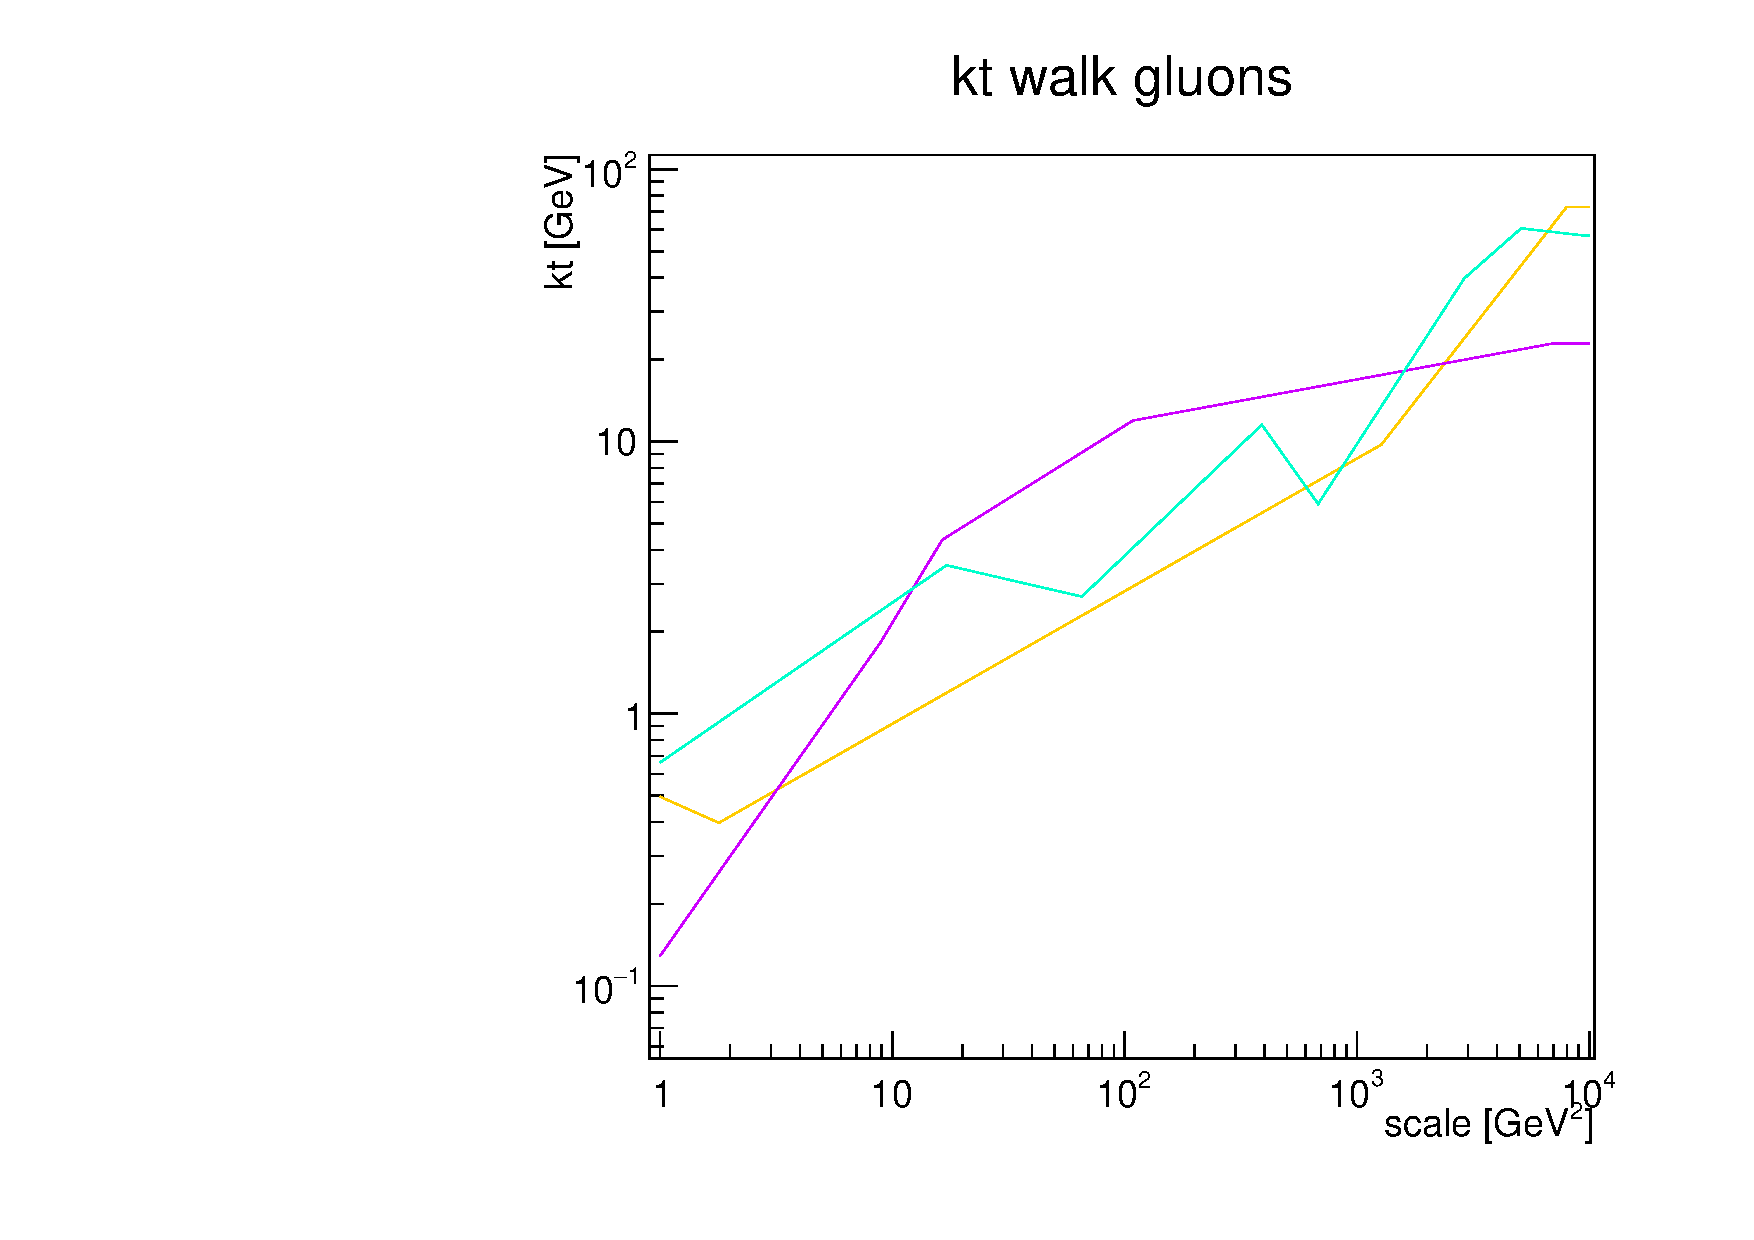
\includegraphics[width=\linewidth]{a-walkskt-Pgg.pdf}
			\caption{sample gluon $k_t$ evolution}
			\label{fig:simp_egkt1}
    \end{subfigure}
    \caption{Evolution process for a sample of three gluon.}
		\label{fig:simp_eg1}
    \end{figure*}

    On \figref{fig:simp_egz1}, we can see the momentum fraction being reduced as splittings occur through 
    the scale evolution. \figref{fig:simp_egkxy1} shows the evolution of the $x$ and $y$ components of 
    the transverse momentum as branchings occur, and \figref{fig:simp_egkt1} plots the $k_t$ with respect to the
    scale. \\

    To get a significant sample, we perform this for $1\,000\,000$ events, and plots the 
    resulting densities in histograms. Note that in order to obtain histograms for the weighted density $xf(x,\mu^2)$, 
    we need to multiply the weight for each $x$ by $x$ itself. There is one last thing to take into account 
    to get the correct normalisation : this method evolves as many partons as that are generated for the initial 
    distribution, but their momentum fraction only lowers. This seems in conflict with the fact 
    that the integral of the momentum density must of course be conserved. It is so because the momentum 
    fraction is not lost, but spread between more partons. To account for this, we must simply normalise 
    the evolved densities to the same momentum integral as the initial ones. We can also note that 
    only the $f(x,\mu^2)$ integrals are conserved through evolution, not the $xf(x,\mu^2)$ nor the $k_t$ ones. 
    (The former because of the shift in the distribution of x, the latter because of the increase of 
    the number of partons : more high-$k_t$ partons does not automatically indicate less low-$k_t$ ones).


    \vfill
    \eject

    \section{Results}

    Here are the resulting histograms : 

    \begin{figure*}[h]
    \centering
    \begin{subfigure}[b]{0.45\linewidth}
      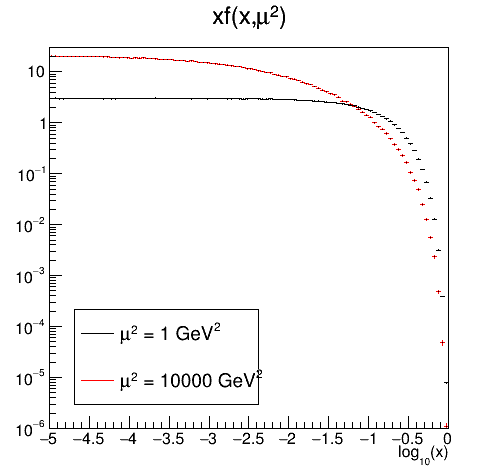
\includegraphics[width=\linewidth]{gg_density_m1.png}
			\caption{gluon density}
			\label{fig:simp_xf1g}
    \end{subfigure}
      \hspace{20pt}
    \begin{subfigure}[b]{0.45\linewidth}
      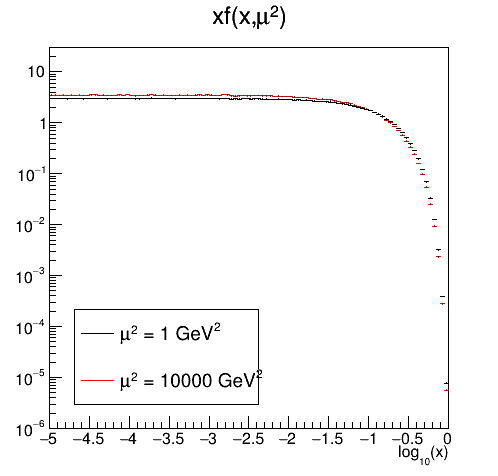
\includegraphics[width=\linewidth]{qq_density_m1.png}
			\caption{quark density}
			\label{fig:simp_xf1q}
    \end{subfigure}
    \caption{Evolution of the momentum weighted parton density.}
		\label{fig:simp_xf1}
    \end{figure*}

    In the gluon case, the migration to small momentum fractions $x$ is plain to see, while in the 
    quark case it is much less pronounced. Seeing the latter, we might fear an inadequacy in the parameters 
    used, perhaps in the cut-off. We will see that the cut-off does play a role, but is also counterbalanced. 
    This result is actually robust, in a sense that we will explore a bit later. The difference between
    the results for the gluon and the quark densities really come from the behaviour of their splitting functions.\\

    Here are the results for the transverse momentum $k_t$ (with angular ordering) : 

    \begin{figure*}[h]
    \centering
    \begin{subfigure}[b]{0.45\linewidth}
      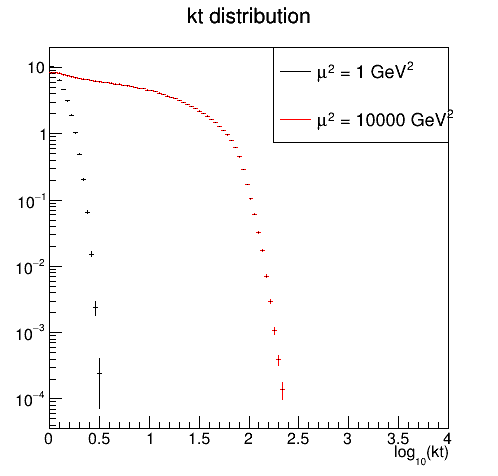
\includegraphics[width=\linewidth]{gg_kt_m1.png}
			\caption{gluon distribution}
			\label{fig:simp_kt1g}
    \end{subfigure}
      \hspace{20pt}
    \begin{subfigure}[b]{0.45\linewidth}
      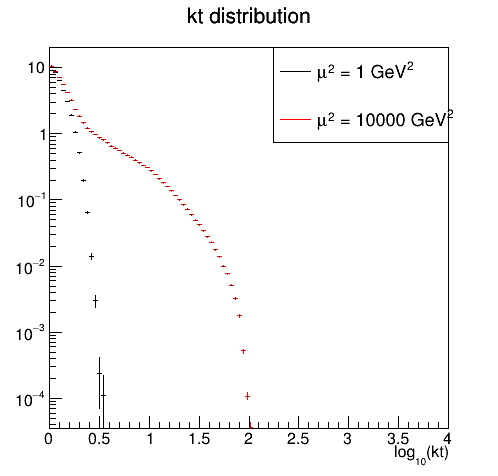
\includegraphics[width=\linewidth]{qq_kt_m1.png}
			\caption{quark distribution}
			\label{fig:simp_kt1q}
    \end{subfigure}
    \caption{Evolution of the transverse momentum distribution.}
		\label{fig:simp_kt1}
    \end{figure*}

    We can notice that the distributions decrease sharply because of the scale limitation, although
    it does exceed it in the gluon case, likely because of the accumulated steps. The quark distribution being
    notably lower might put in conjunction with the less pronounced evolution, but the abrupt stop at the 
    final scale might indicate that hardly more than one branching ever occur for a single event.\\

    This justifies an investigation on the dependence of these results on, say, the cut-off $\epsilon$, 
    which gives $z_{min} = \epsilon,\, z_{max}=1-\epsilon$ and thus control the integrals on the splitting function.\\

    Let us take a look at the $\epsilon$ dependence for the scale generation : 

    \begin{figure*}[h]
    \centering
    \begin{subfigure}[b]{0.45\linewidth}
      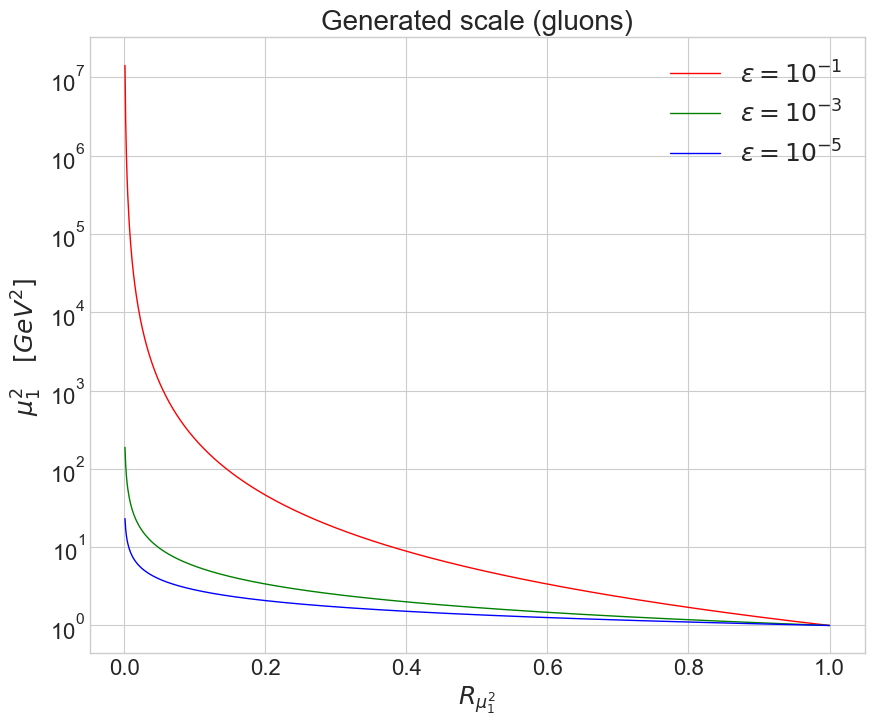
\includegraphics[width=\linewidth]{genscalege.png}
			\caption{gluon case}
			\label{fig:simp_gmu1g}
    \end{subfigure}
      \hspace{20pt}
    \begin{subfigure}[b]{0.45\linewidth}
      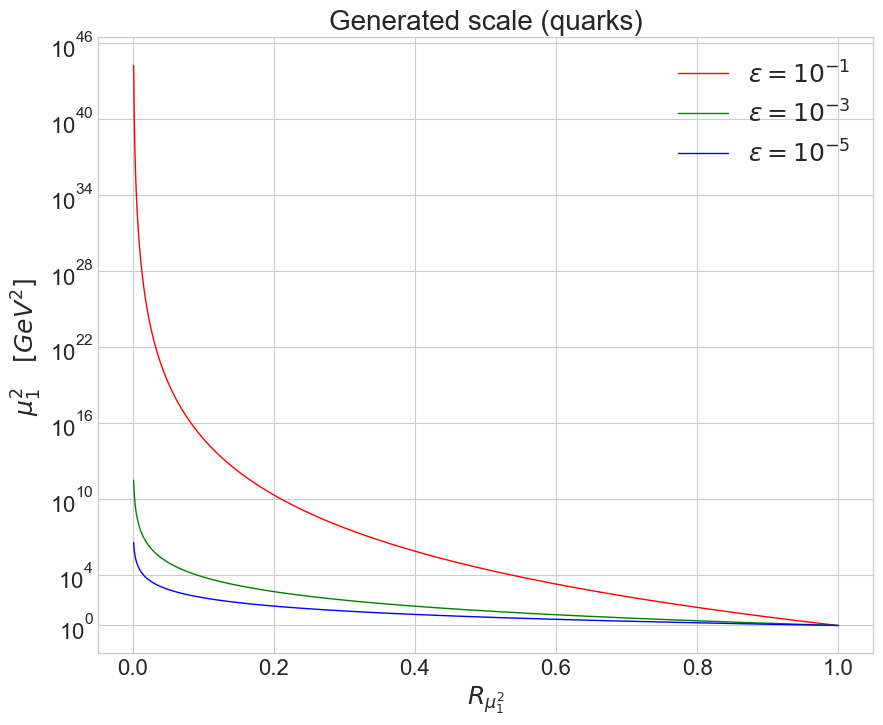
\includegraphics[width=\linewidth]{genscaleqe.png}
			\caption{quark case}
			\label{fig:simp_gmu1q}
    \end{subfigure}
    \caption{First generated scale $\mu_1^2$ with respect to the random number $R_{\mu_1^2}$, depending on $\epsilon$.}
		\label{fig:simp_gmu1}
    \end{figure*}

    Let us recall that the evolution is stopped when $\mu_i^2>\mu_f^2\equiv10^4\,\text{GeV}^2$. Let us also recall 
    that from \equref{eq:simp_scalegen}, with a different initial scale $\mu_0^2 \neq 1$ we would 
    have got the same graph, with $\mu_1^2$ multiplied by $\mu_0^2$.\\
    We can see that decreasing $\epsilon$ decrease the probability of generating large scales (a smaller 
    range of $R_{\mu_1^2}$ would produce them), which overall 
    means that there will be more branching before the final scale is reached. We can also note 
    that the scales generated in the quark case are often very large, especially for $\epsilon = 0.1$.
    In this latter case, for more than half the events, no branching would occur at all (as for 
    $R_{\mu_1^2} \in (0, 0.54)$, we have $\mu_1^2 > \mu_f^2$).\\ 

    Let us have a look at how $\epsilon$ affects the density plots : 

    \begin{figure*}[h]
    \centering
    \begin{subfigure}[b]{0.45\linewidth}
      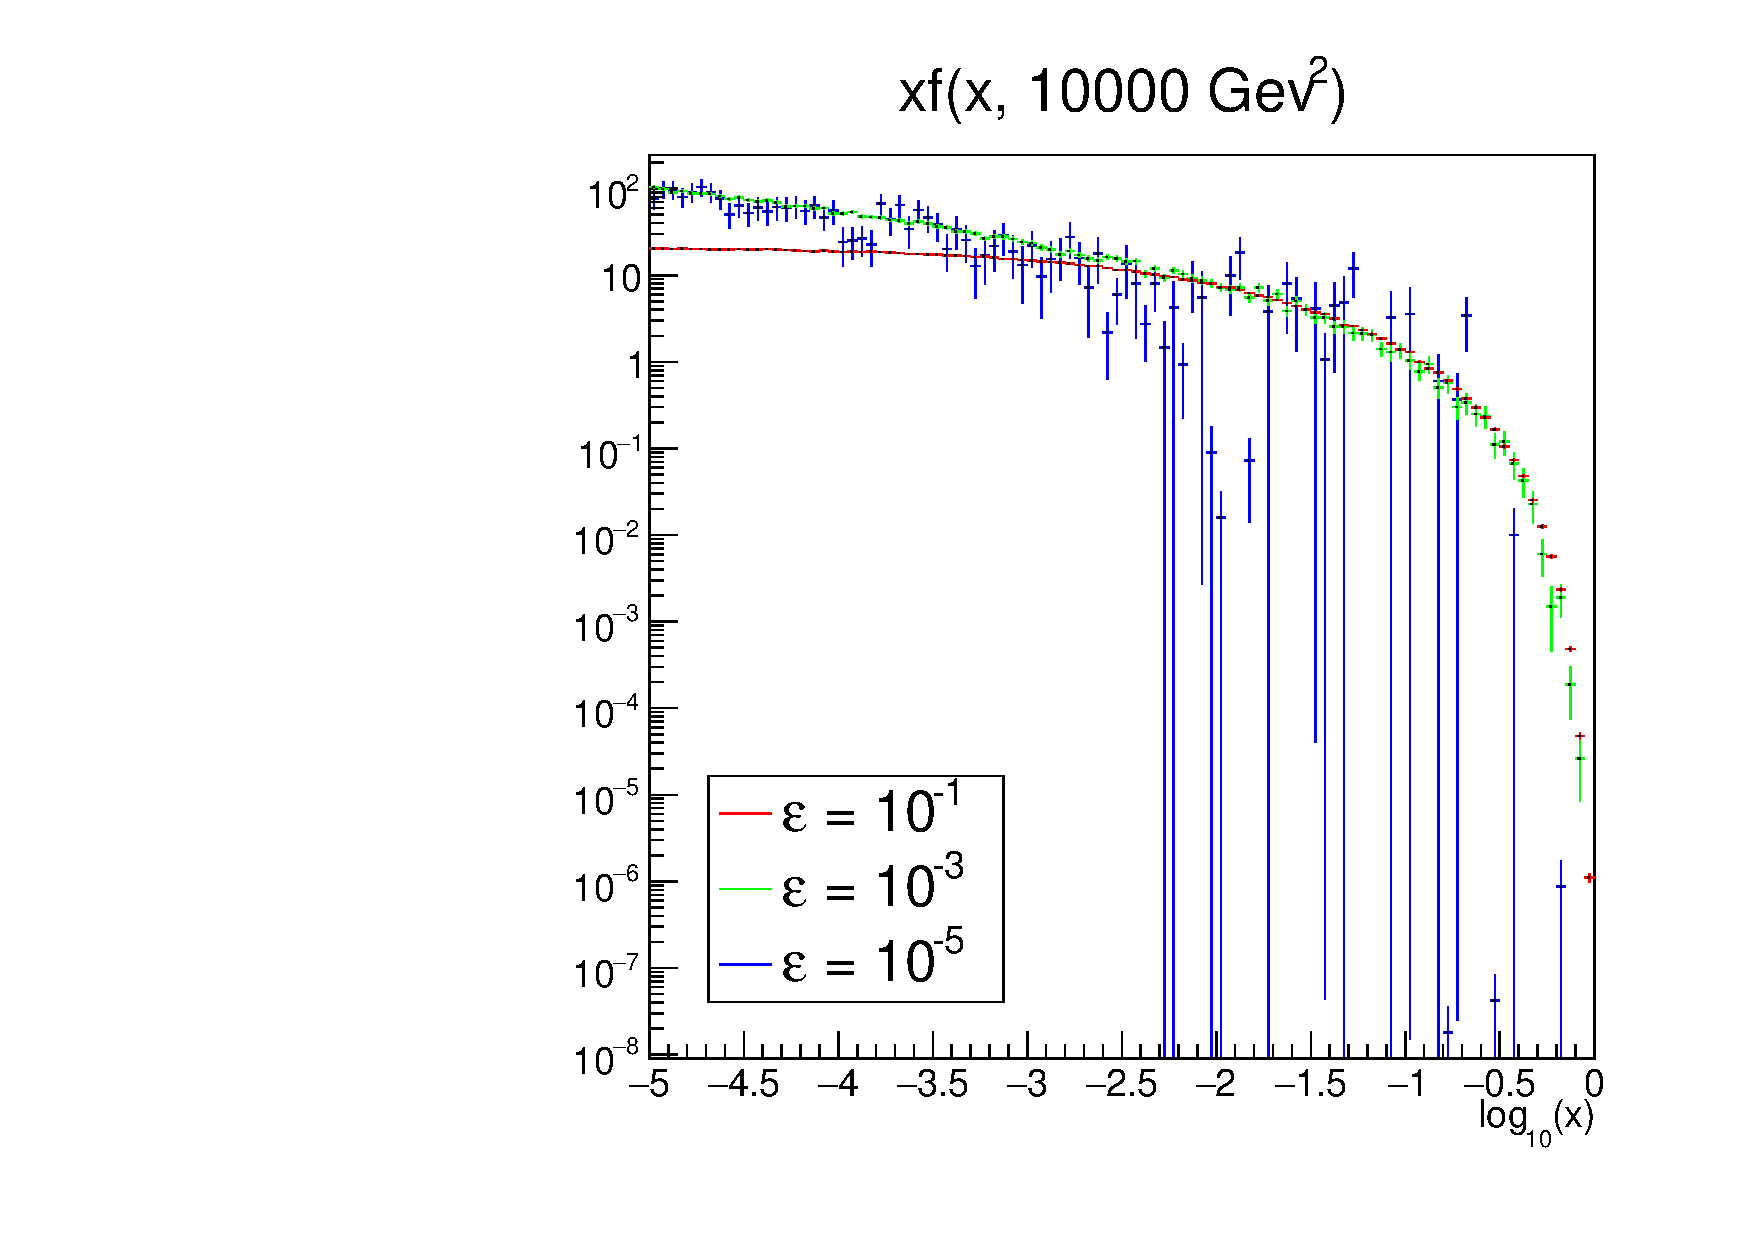
\includegraphics[width=\linewidth]{gg_density_mms.pdf}
			\caption{gluon density}
			\label{fig:simp_xf2g}
    \end{subfigure}
      \hspace{20pt}
    \begin{subfigure}[b]{0.45\linewidth}
      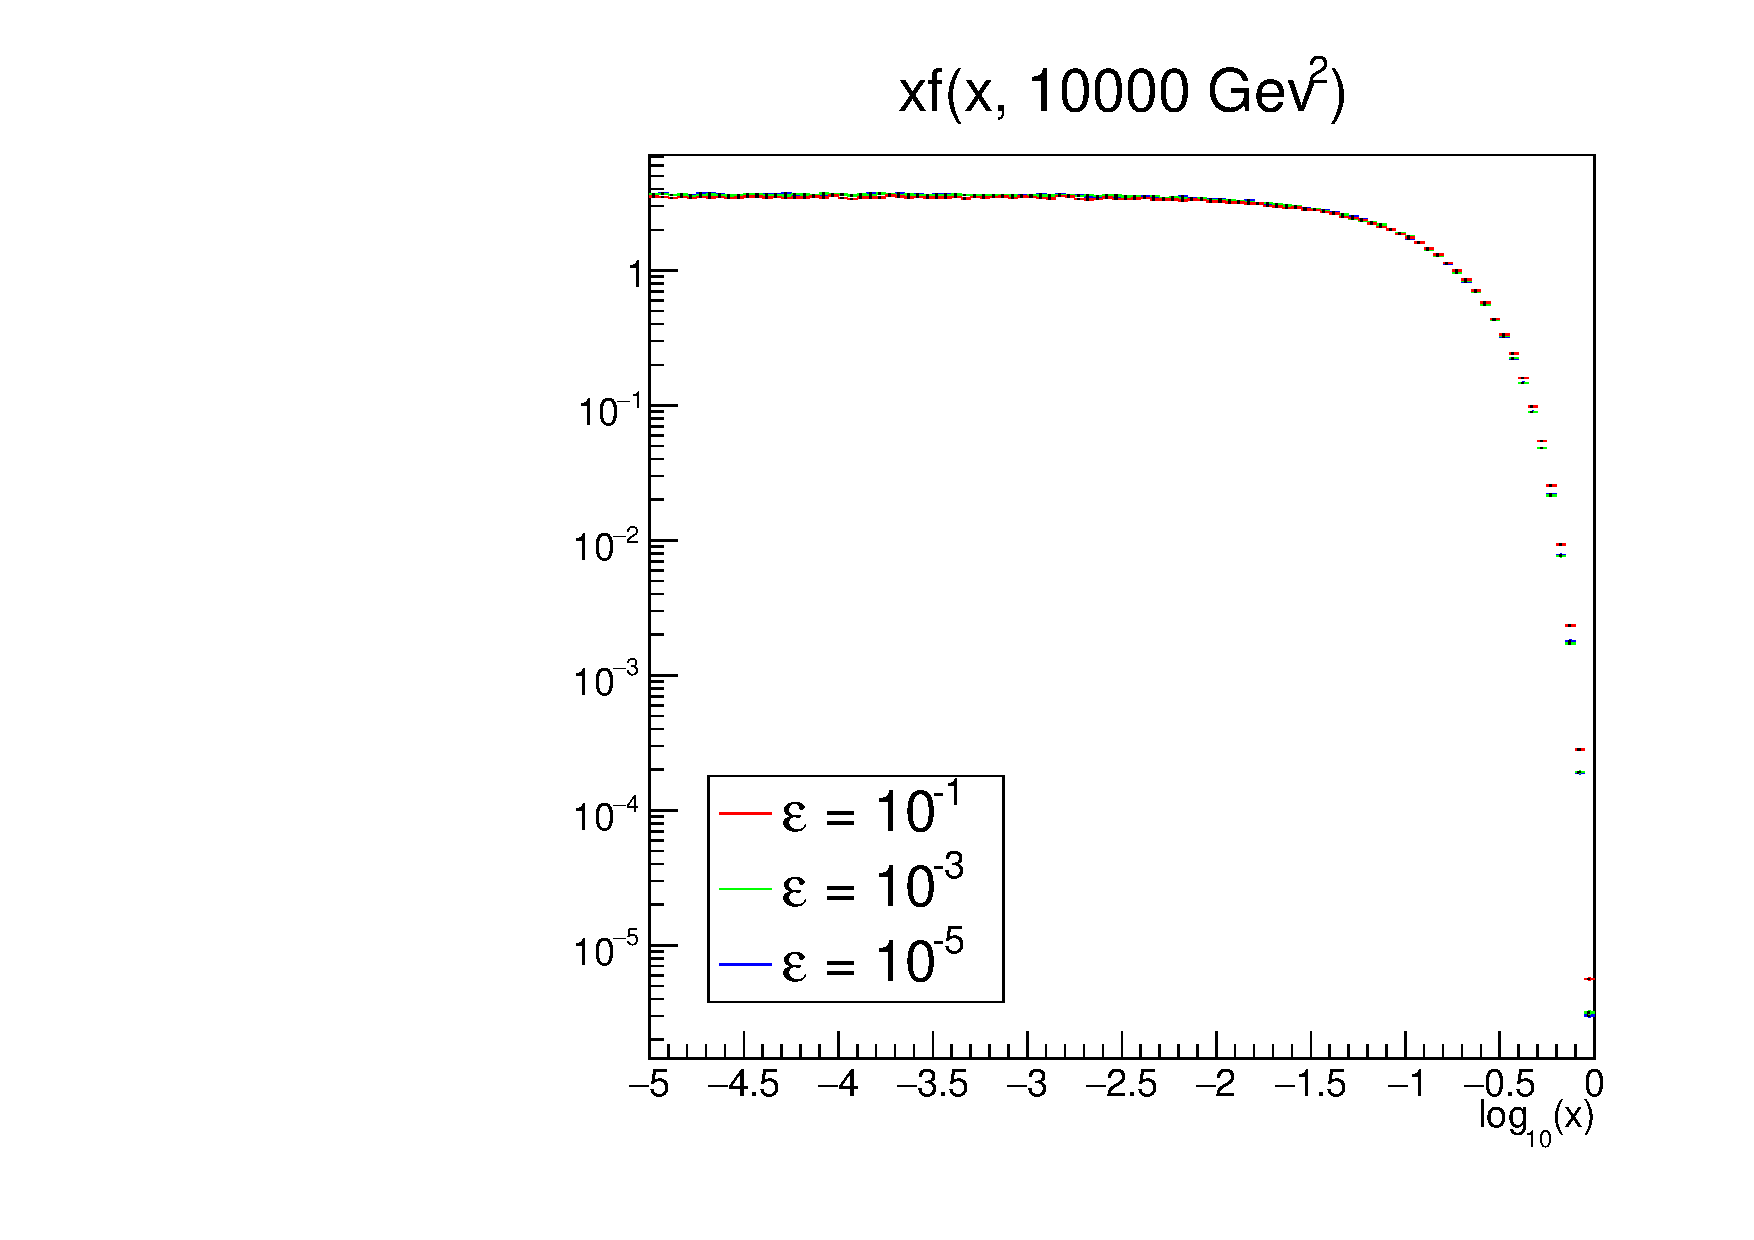
\includegraphics[width=\linewidth]{qq_density_mms.pdf}
			\caption{quark density}
			\label{fig:simp_xf2q}
    \end{subfigure}
    \caption{Evolved momentum weighted parton density, depending on $\epsilon$.}
		\label{fig:simp_xf2}
    \end{figure*}

    The gluon density is strongly affected : decreasing $\epsilon$ strongly increase the density for small 
    momentum fractions. \\
    \textit{\textbf{Note :} The $\epsilon = 10^{-5}$ case is messy because of scarcely 
    filled bins : on $1\,000\,000$ events generated, only 76 end up in the right half of the plot (the majority is actually 
    in the underflow).}\\
    Perhaps surprisingly, the quark density seems mostly unaffected by the variation of $\epsilon$. We need 
    to look at the $k_t$ distribution to find a difference : 

    \begin{figure*}[h]
    \centering
    \begin{subfigure}[b]{0.45\linewidth}
      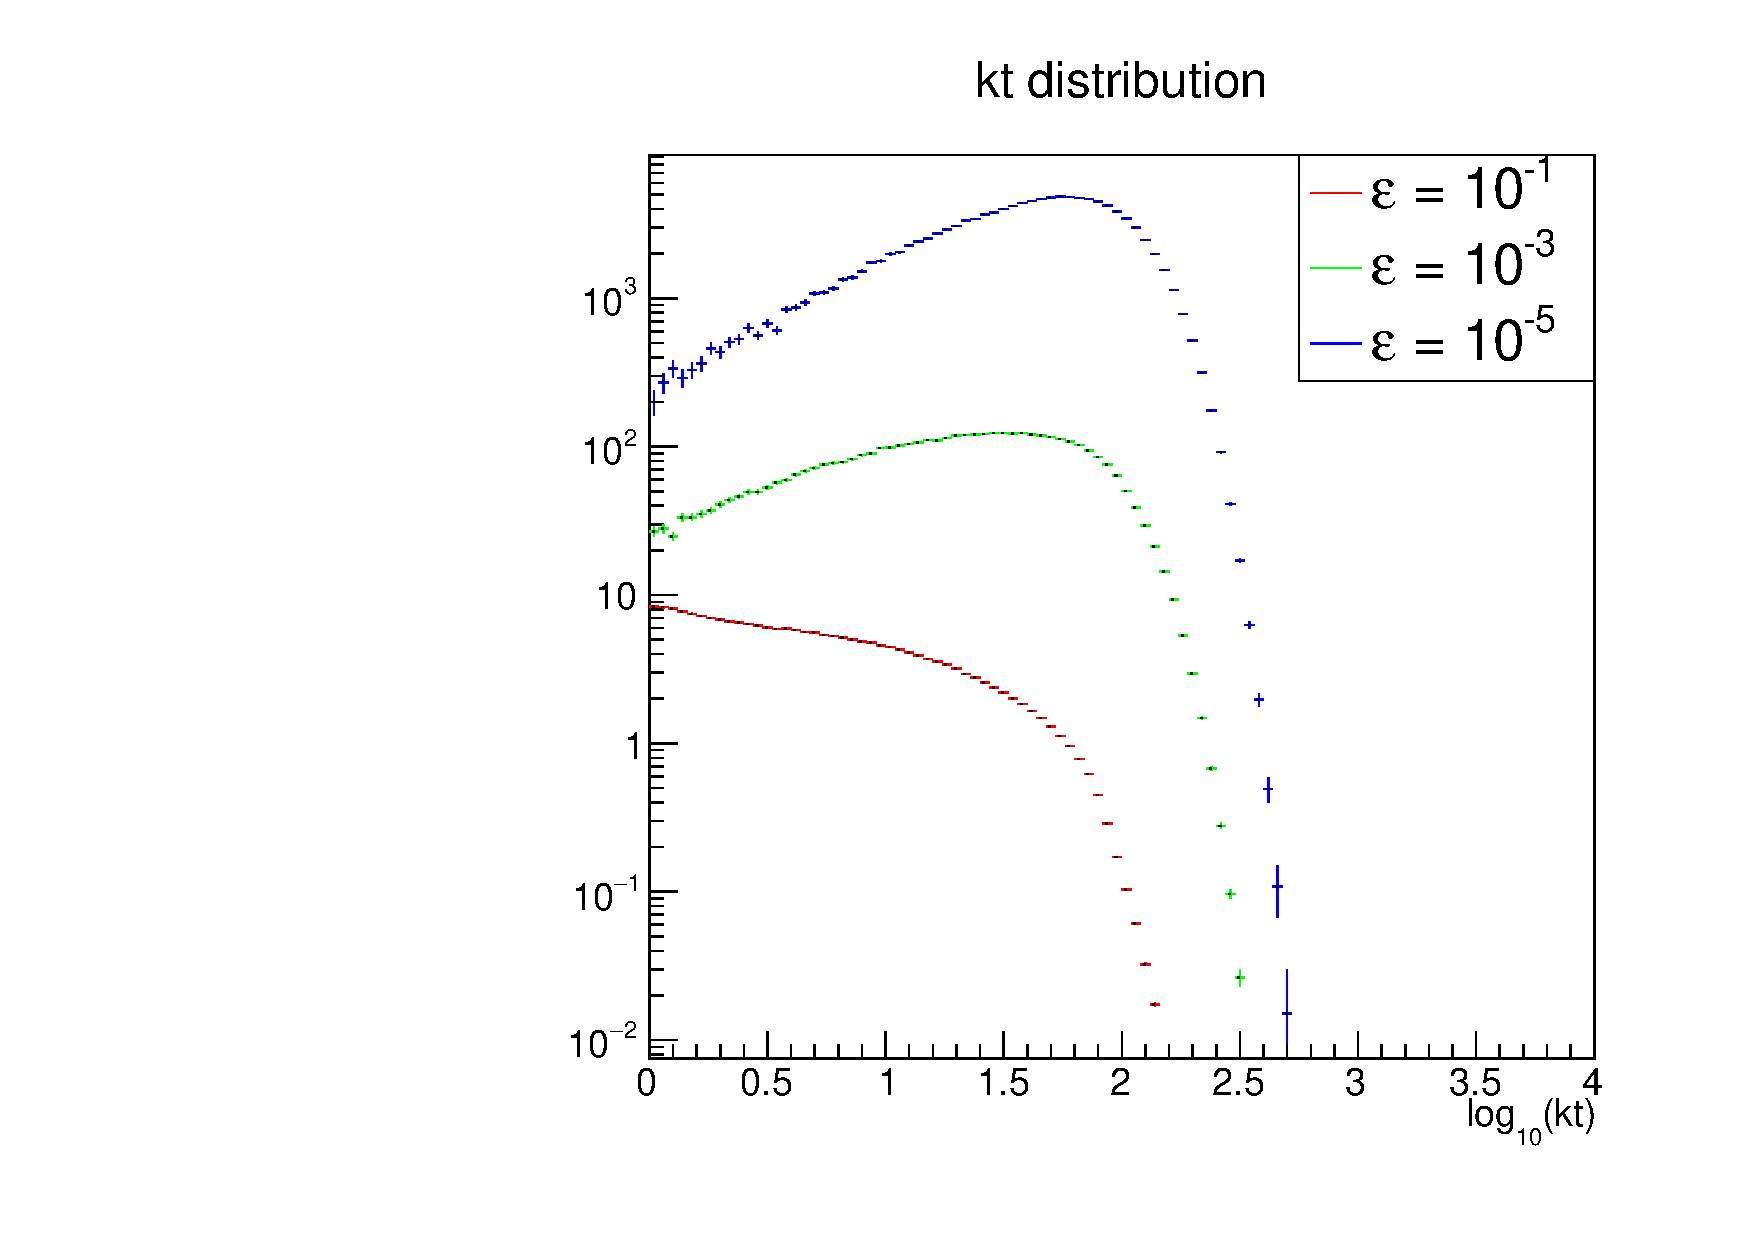
\includegraphics[width=\linewidth]{gg_kt_mms.pdf}
			\caption{gluon distribution}
			\label{fig:simp_kt2g}
    \end{subfigure}
      \hspace{20pt}
    \begin{subfigure}[b]{0.45\linewidth}
      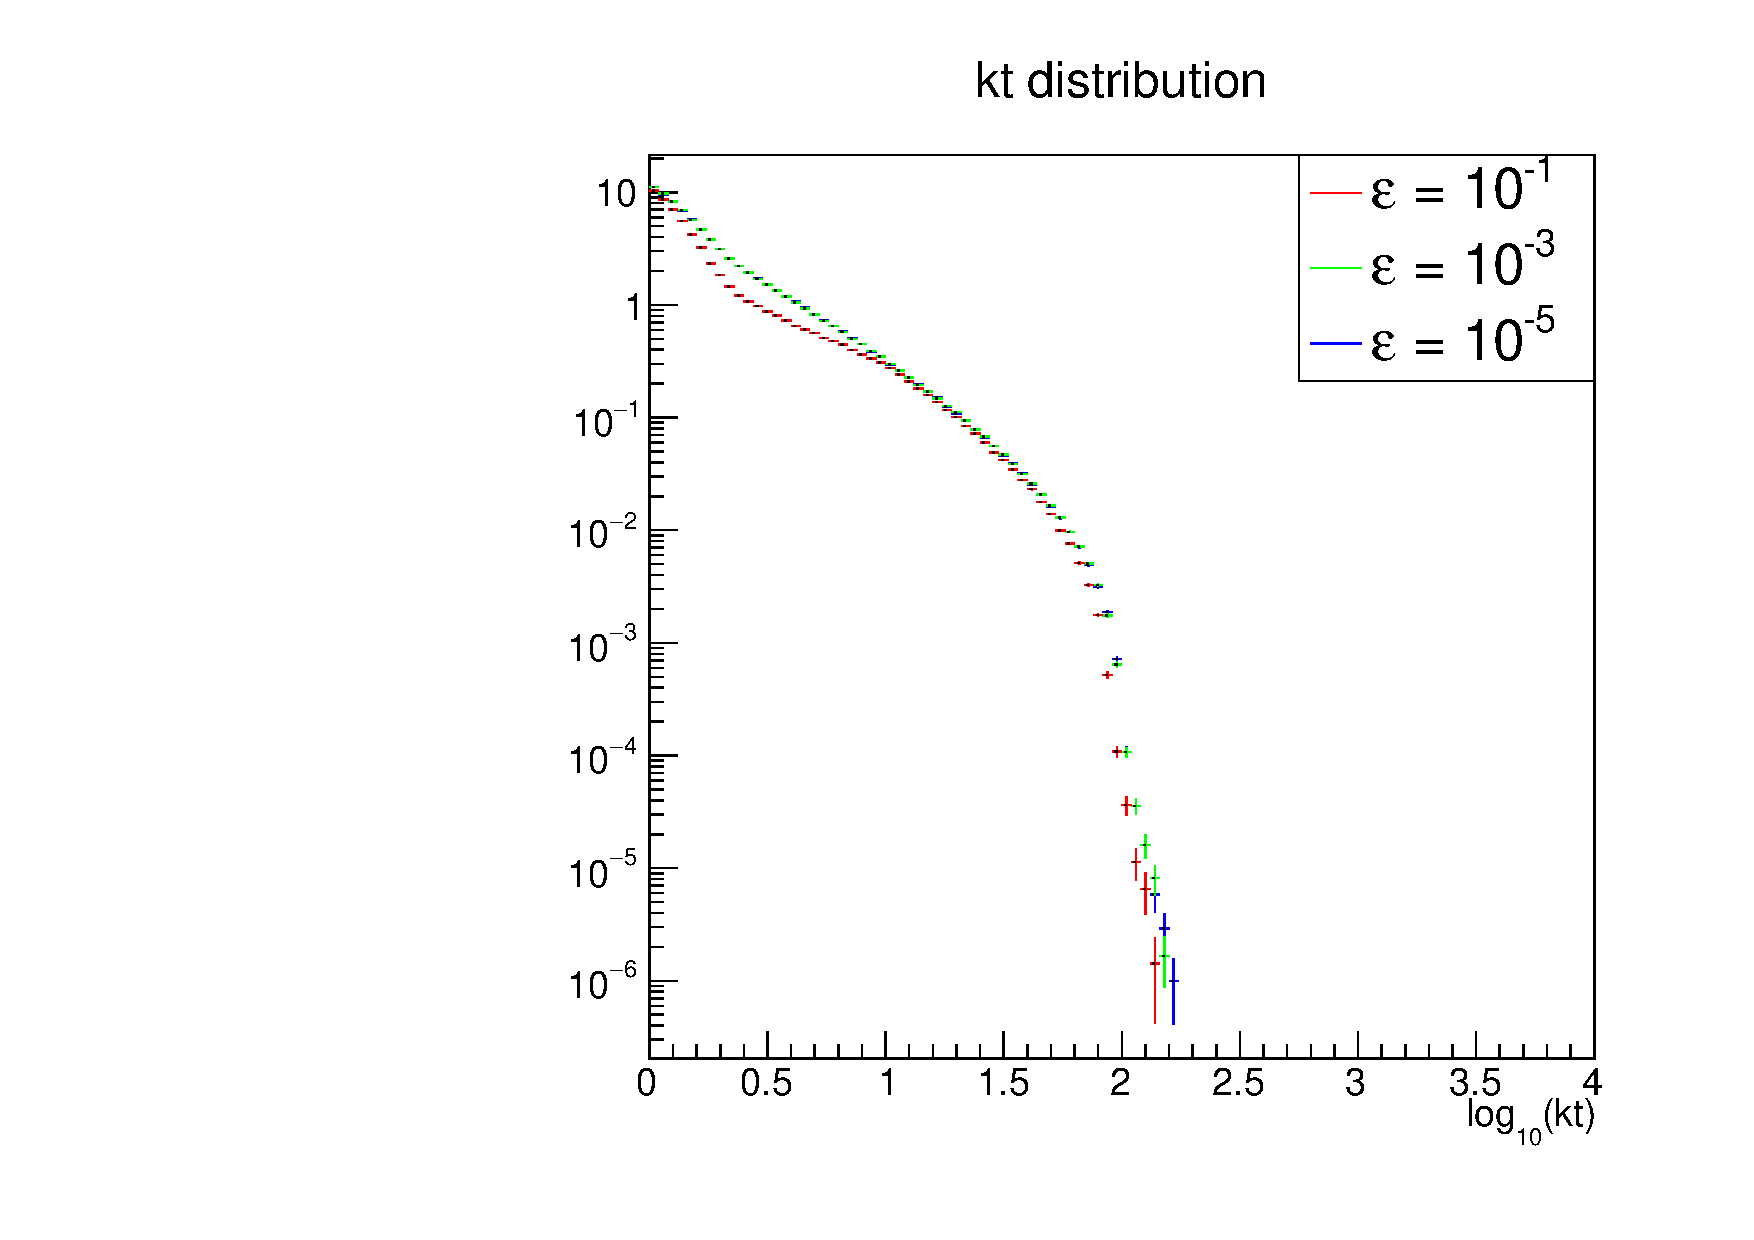
\includegraphics[width=\linewidth]{qq_kt_mms.pdf}
			\caption{quark distribution}
			\label{fig:simp_kt2q}
    \end{subfigure}
    \caption{Evolved transverse momentum distribution, depending on $\epsilon$.}
		\label{fig:simp_kt2}
    \end{figure*}

    The gluon density is still strongly affected, while for the quark density, the $\epsilon = 10^{-3}$ and 
    $\epsilon = 10^{-5}$ straighten up a bit from the $\epsilon = 10^{-1}$ case, but match with each other. 
    We can suppose that with $\epsilon$ to large, there weren't quite enough branchings generated to get a 
    statistically sound $k_t$ distribution, while the quark distribution otherwise don't seem to depend on it. 
    This is not the case for the gluon distributions. To understand this better, we need to take a look at the 
    $\epsilon$ dependence of the splitting variable generation : 

    \begin{figure*}[h]
    \centering
    \begin{subfigure}[b]{0.45\linewidth}
      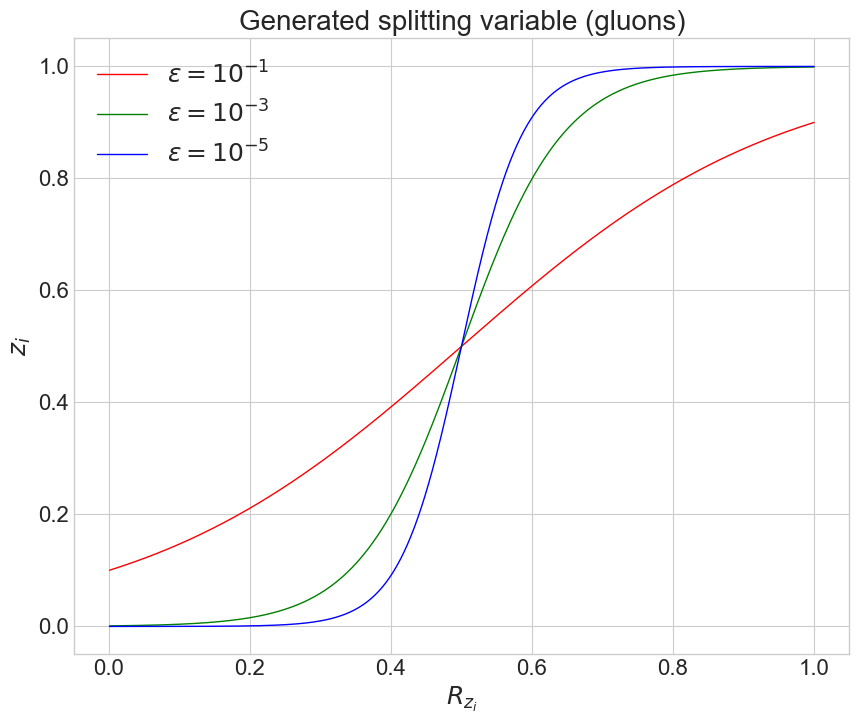
\includegraphics[width=\linewidth]{gensplige.png}
			\caption{gluon case}
			\label{fig:simp_gz1g}
    \end{subfigure}
      \hspace{20pt}
    \begin{subfigure}[b]{0.4\linewidth}
      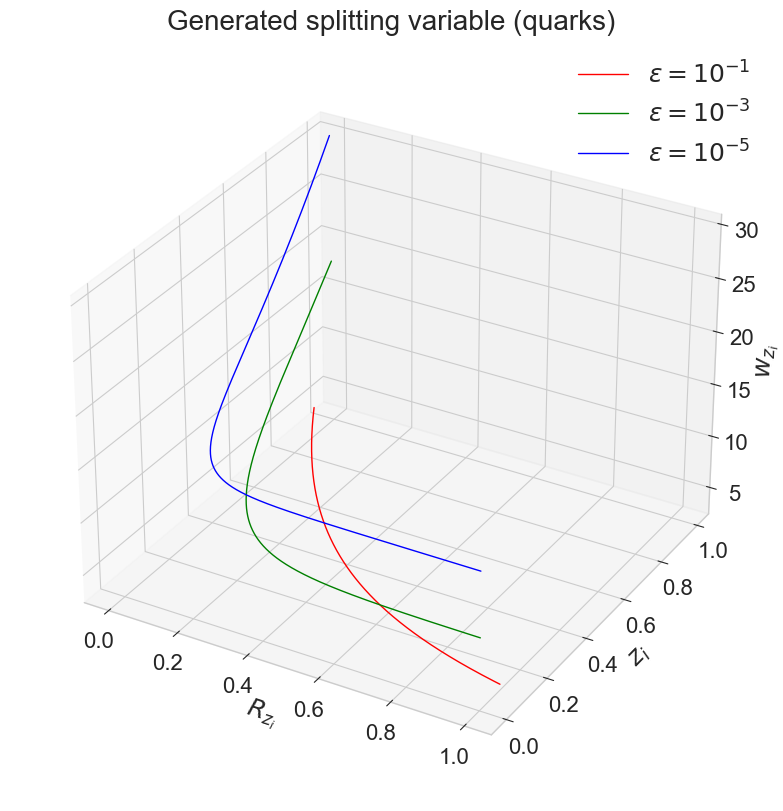
\includegraphics[width=\linewidth]{genspliqe.png}
			\caption{quark case, showing the weights}
			\label{fig:simp_gz1q}
    \end{subfigure}
    \caption{Generated splitting variable $z_i$ with respect to the random number $R_{z_i}$, depending on $\epsilon$.}
		\label{fig:simp_gz1}
    \end{figure*}

    Since we used the importance sampling method to generate the quark splitting, we need to show the corresponding weights 
    to accurately display the importance of each value in the results. We can notice that for the quark case, reducing 
    $\epsilon$ increase the importance of large $z_i$ values. Thus events where the splittings doesn't change the momentum 
    fraction much ($z$ close to 1) weight more in the histogram, while, as seen in \figref{fig:simp_gmu1}, more 
    branchings occur and produce more splittings, reducing $x$ more. Apparently, these two opposite effects 
    cancel each other in the quark case, giving $\epsilon$-independant results (provided $\epsilon$ is not \textit{too} large). 
    This is quite fortunate, since the cut-off is unphysical.\\ 
    We are not so lucky with the gluon density, but we can see why in \figref{fig:simp_gz1g} : decreasing 
    $\epsilon$ makes $z_i$ close to 1 more probable, but also $z_i$ close to 0. This latter effect explain the 
    strong migration towards very small momentum fractions in \figref{fig:simp_xf2g}.
    We also generate more splittings, and given the formula for the $k_t$ used in \equref{eq:simp_angord}, we make 
    more large jumps in $k_t$, which explains the large density for large $k_t$ in \figref{fig:simp_kt2g}.\\ 
    Compared to \figref{fig:simp_eg1}, we now get more events like these :

    \begin{figure*}[h]
    \centering
    \begin{subfigure}[b]{0.31\linewidth}
      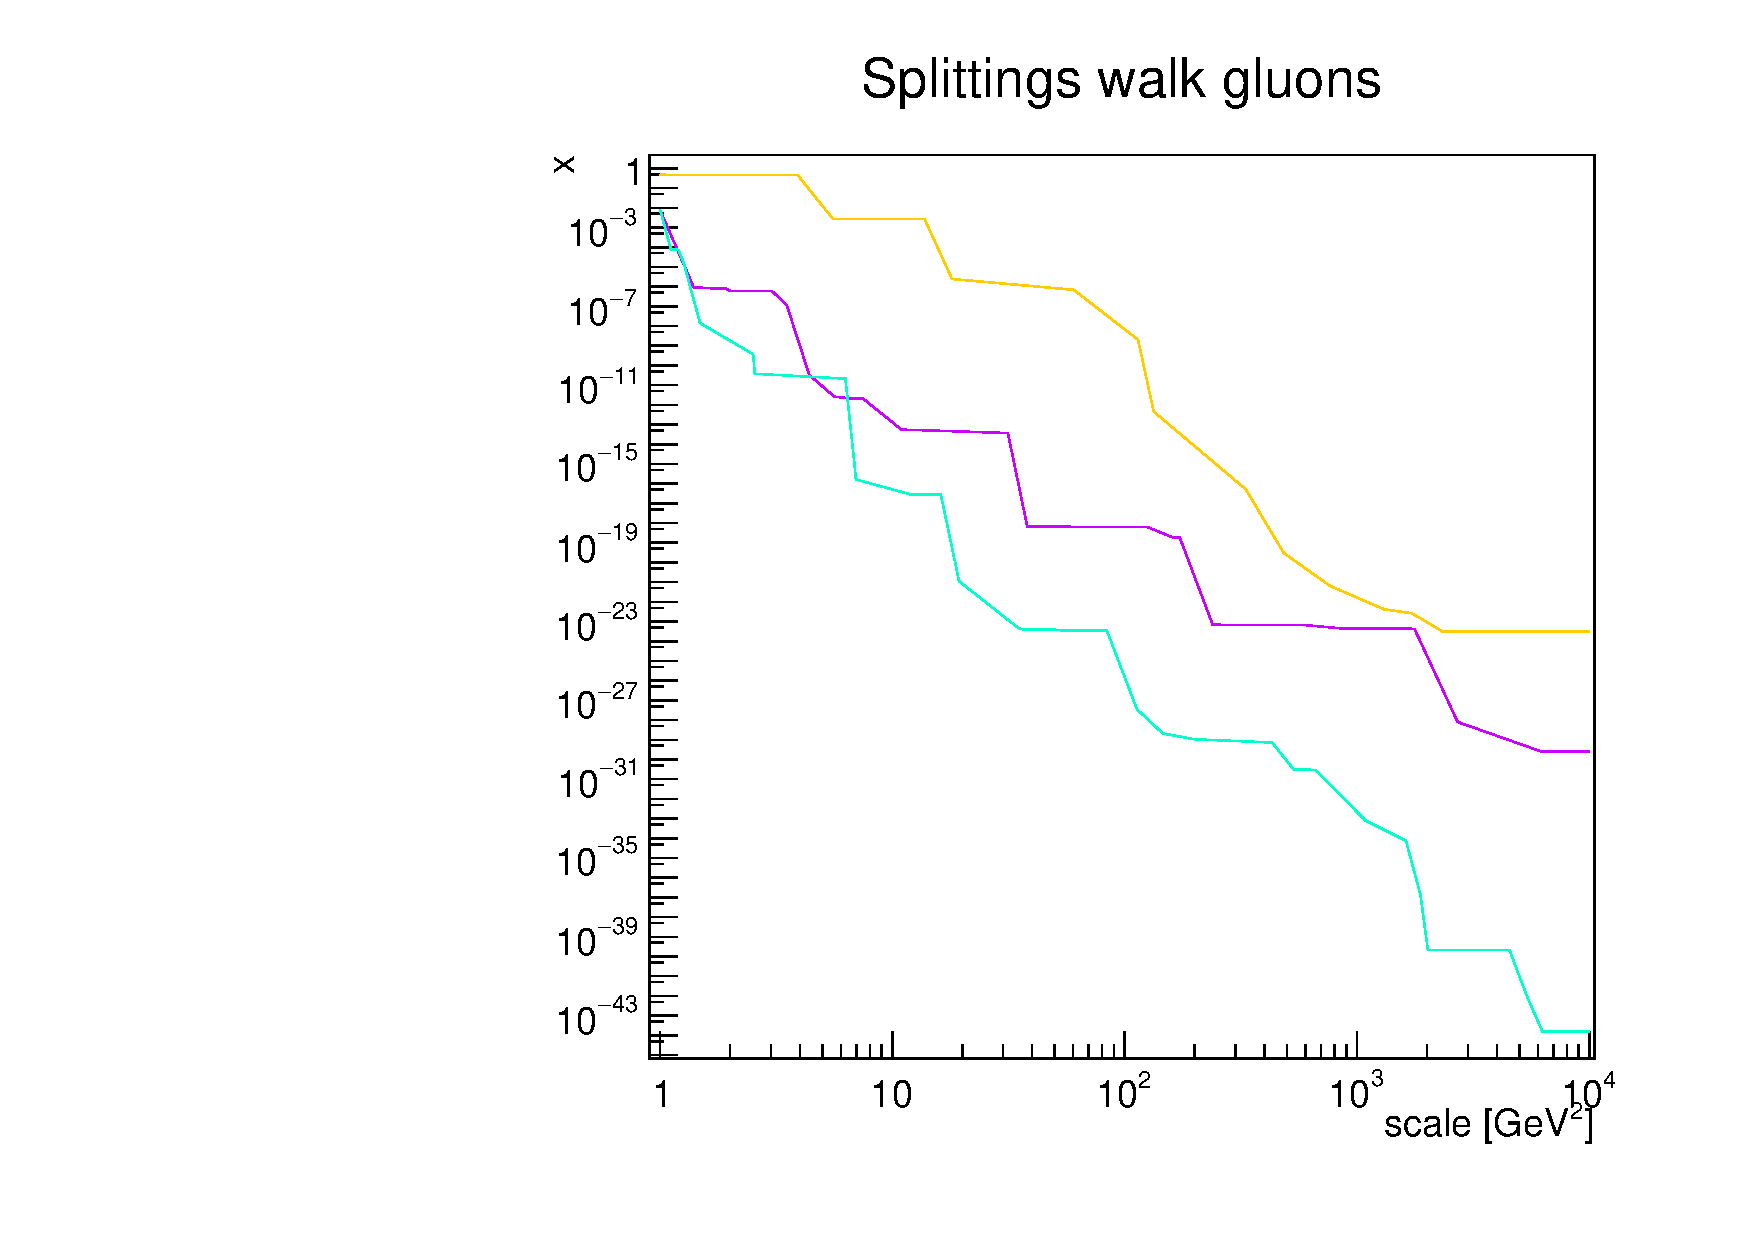
\includegraphics[width=\linewidth]{a-walksz-Pgge5.pdf}
			\caption{$\epsilon = 10^{-5}$ gluon evolution}
			\label{fig:simp_egz2}
    \end{subfigure}
      \hspace{10pt}
    \begin{subfigure}[b]{0.31\linewidth}
      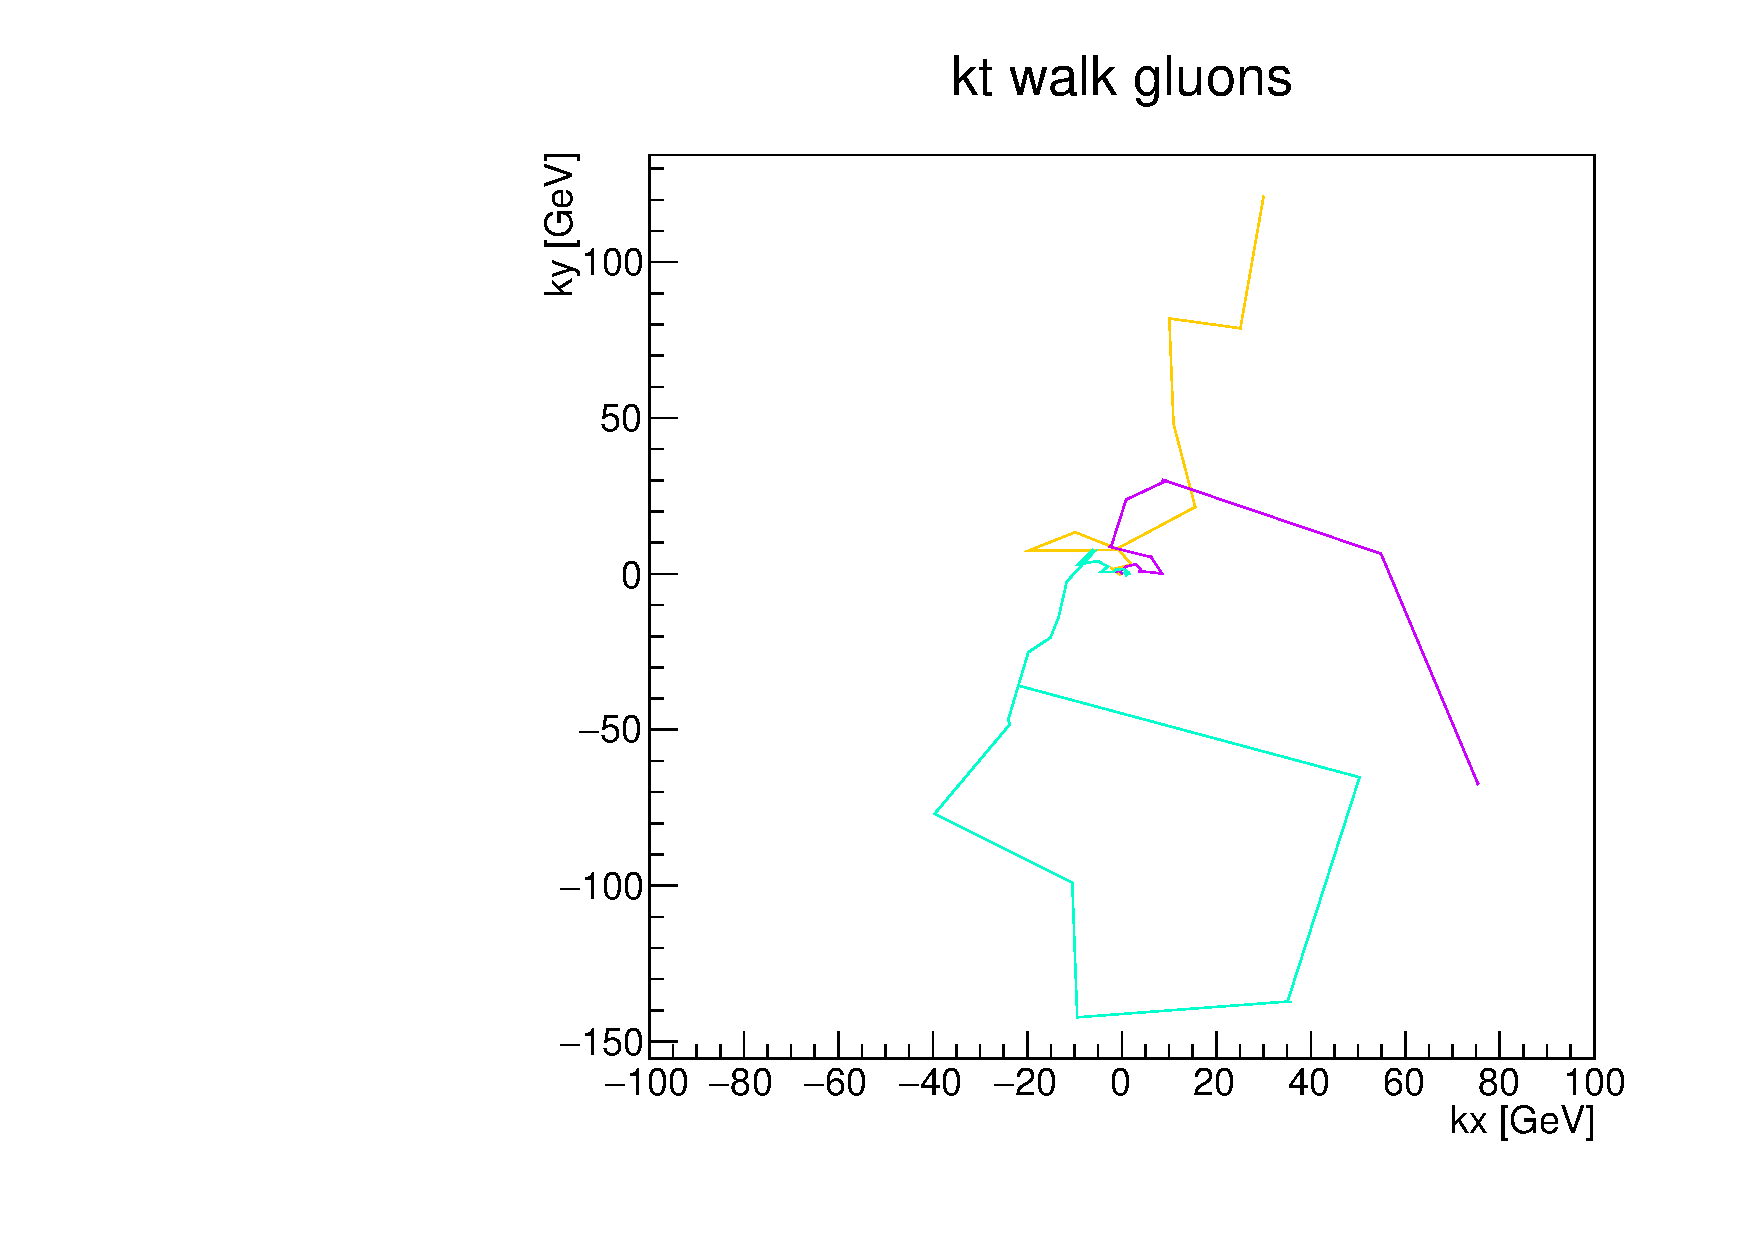
\includegraphics[width=\linewidth]{a-walksktxy-Pgge5.pdf}
			\caption{$\epsilon = 10^{-5}$ gluon $k_t$ generation}
			\label{fig:simp_egkxy2}
    \end{subfigure}
      \hspace{10pt}
    \begin{subfigure}[b]{0.31\linewidth}
      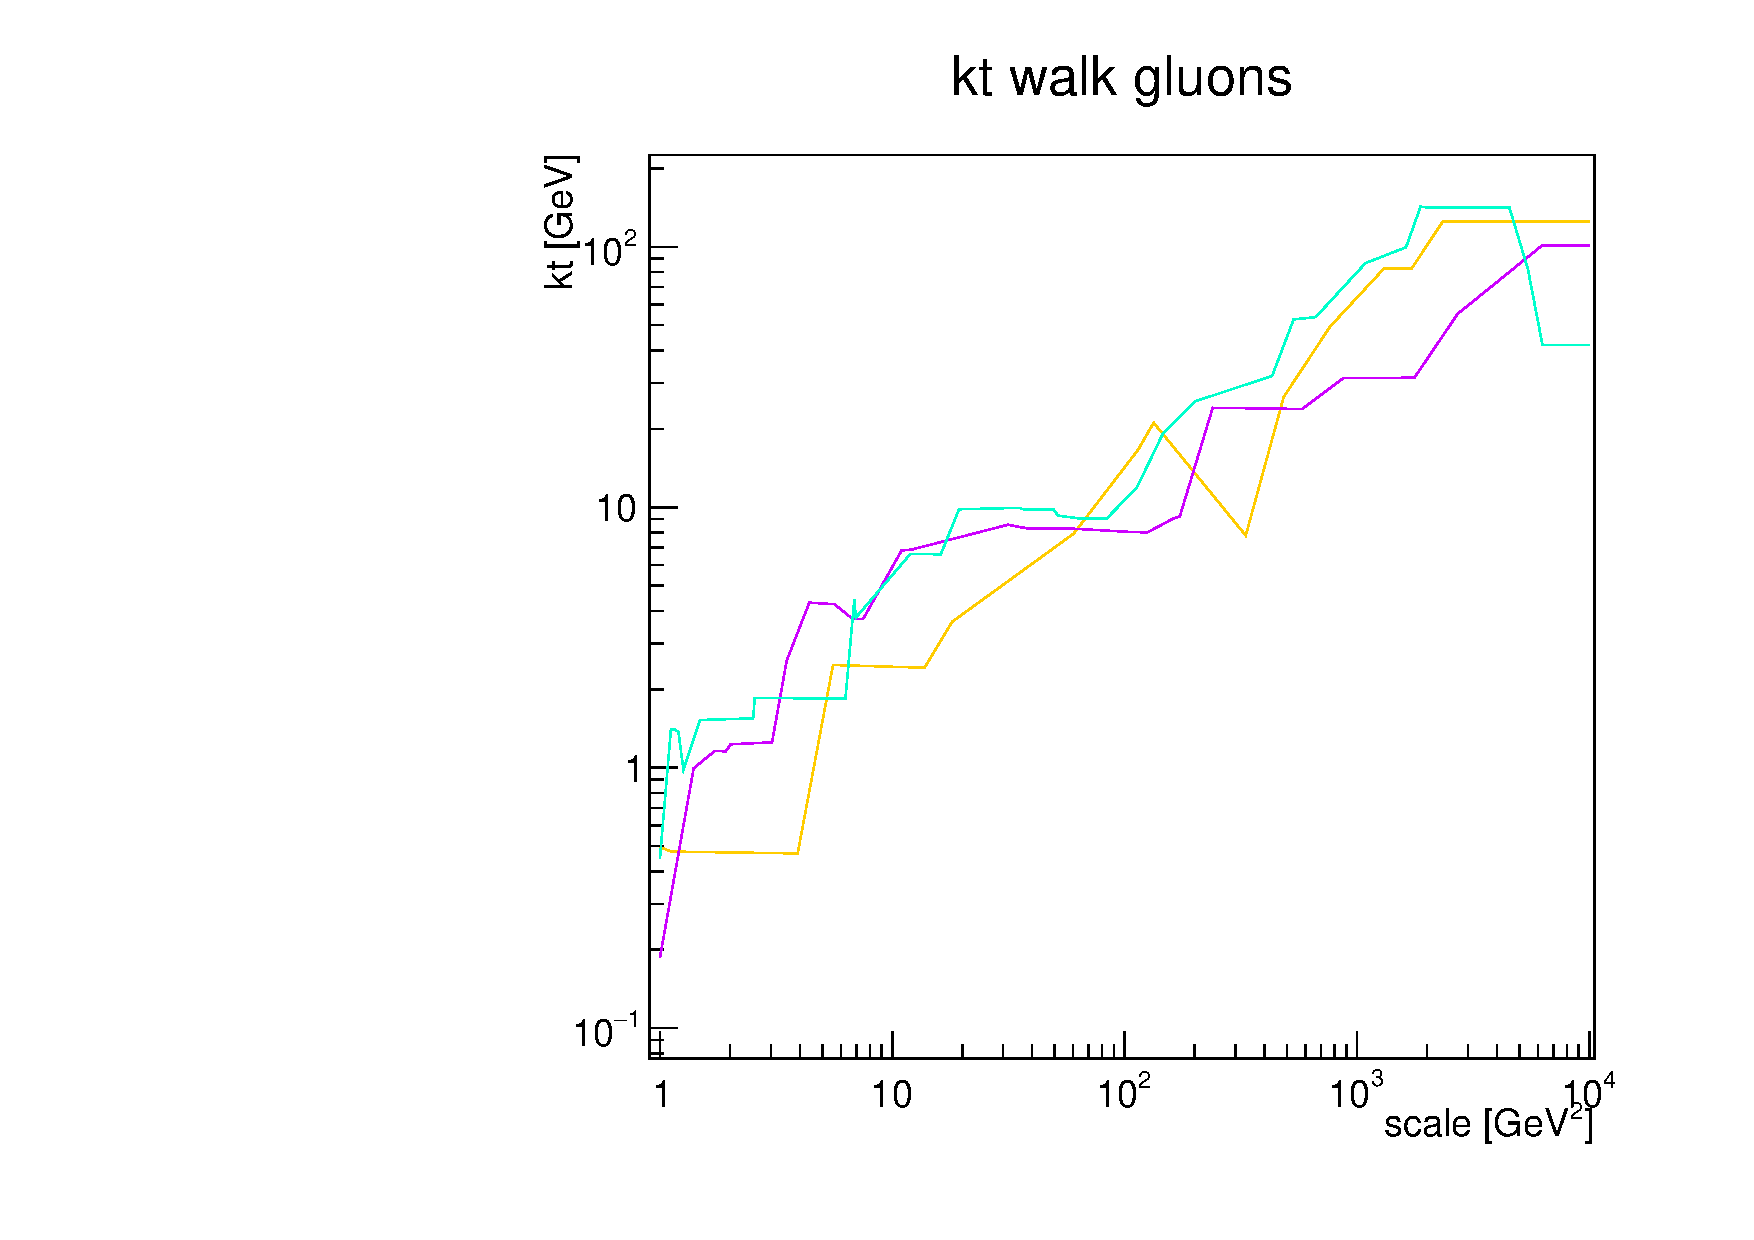
\includegraphics[width=\linewidth]{a-walkskt-Pgge5.pdf}
			\caption{$\epsilon = 10^{-5}$ gluon $k_t$ evolution}
			\label{fig:simp_egkt2}
    \end{subfigure}
    \caption{Evolution process for a sample of three gluon, with $\epsilon = 10^{-5}$.}
		\label{fig:simp_eg2}
    \end{figure*}    

    These events exemplify well the behaviour discussed : we can see on \figref{fig:simp_egz2} a 
    lot of splitting who sharply decrease the momentum fraction, and on the remaining plots, 
    the tendency to build a large $k_t$.\\

    We can then ask ourselves how would this turn out if we fixed $z_{min}$, in hope to avoid this small $z_i$ issue.
    With $z_{min} = 0.1$ fixed, the variable generation would then behave this way : 

    \begin{figure*}[h]
    \centering
    \begin{subfigure}[b]{0.45\linewidth}
      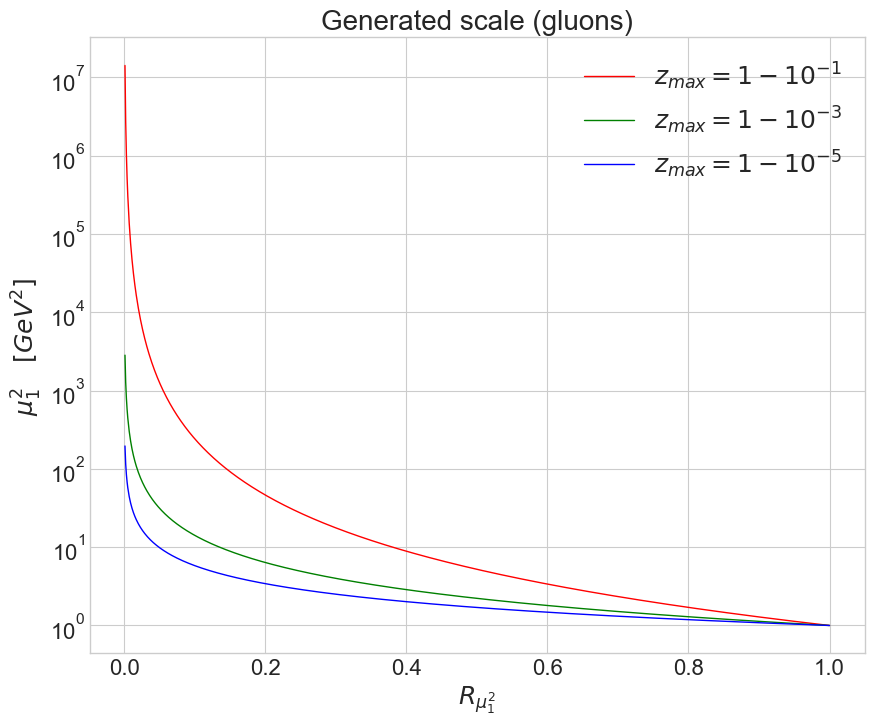
\includegraphics[width=\linewidth]{genscalegz.png}
			\caption{gluon case}
			\label{fig:simp_gmu2g}
    \end{subfigure}
      \hspace{20pt}
    \begin{subfigure}[b]{0.45\linewidth}
      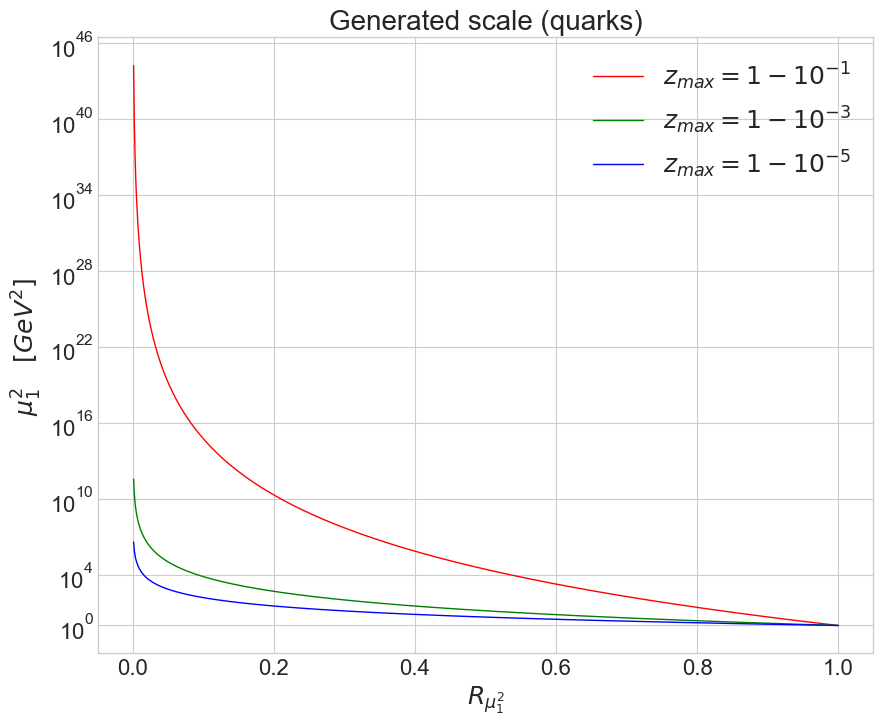
\includegraphics[width=\linewidth]{genscaleqz.png}
			\caption{quark case}
			\label{fig:simp_gmu2q}
    \end{subfigure}
    \caption{First generated scale $\mu_1^2$ with respect to $R_{\mu_1^2}$, fixed $z_{min}$, variable $z_{max}$.}
		\label{fig:simp_gmu2}
    \end{figure*}

    The generation of the scale is noticeably changed only for the gluon case. This is natural, as 
    the splitting function for the gluon in \equref{eq:simp_pgg} diverge as $z \rightarrow 0$, while it is not 
    the case for the quark in \equref{eq:simp_pqq}. By fixing $z_{min}$, we avoid this divergent contribution. 
    So now we have more chances to generate bigger scales, compared to the unfixed $z_{min}$ scales, 
    so we shouldn't get as many splittings per events as we could see in \figref{fig:simp_egz2}. 
    (To be clear, approaching $z_{max}$ of 1 still increases the amount of splittings, just not as much 
    as when we approached $z_{min}$ from 0 too.)\\
    The change for gluons is especially striking for the splitting variable generation :

    \begin{figure*}[h]
    \centering
    \begin{subfigure}[b]{0.45\linewidth}
      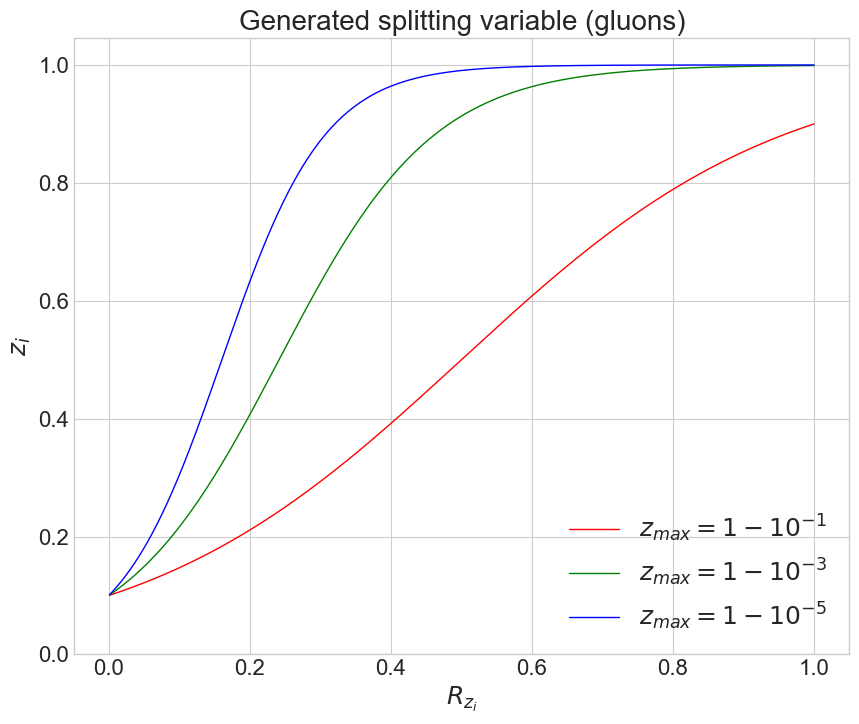
\includegraphics[width=\linewidth]{genspligz.png}
			\caption{gluon case}
			\label{fig:simp_gz2g}
    \end{subfigure}
      \hspace{20pt}
    \begin{subfigure}[b]{0.4\linewidth}
      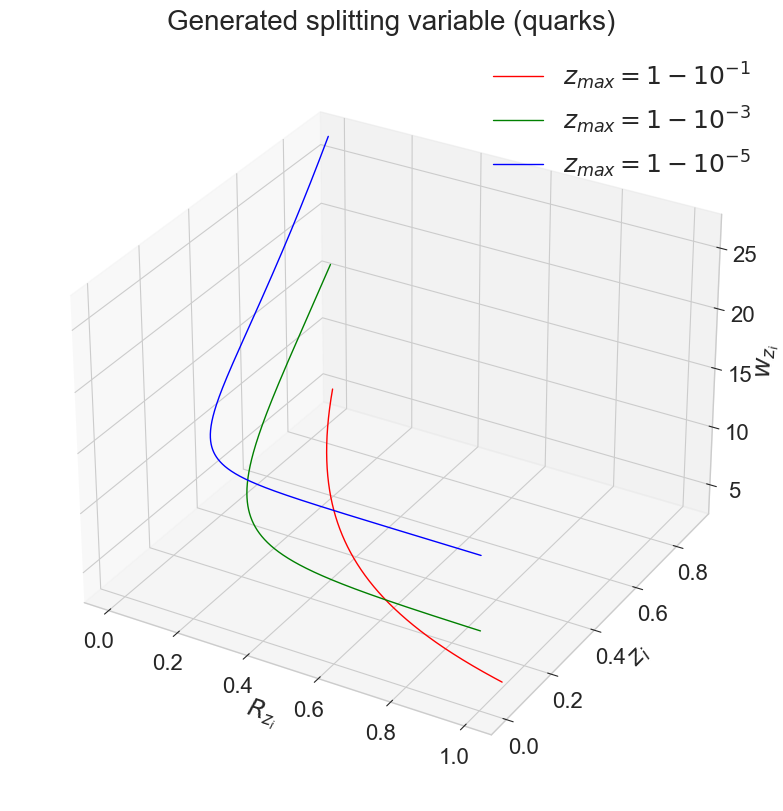
\includegraphics[width=\linewidth]{genspliqz.png}
			\caption{quark case, showing the weights}
			\label{fig:simp_gz2q}
    \end{subfigure}
    \caption{Generated splitting variable $z_i$ with respect to $R_{z_i}$, fixed $z_{min}$, variable $z_{max}$.}
		\label{fig:simp_gz2}
    \end{figure*}

    Now, we can't generate $z$ values arbitrarily close to zero, and small values are becoming less likely as we take $z_{max}$ 
    closer to 1. The splittings will then be less impactful.\\
    For the quarks, the biggest change is in the weight, but it is proportional for each case. Fixing 
    $z_{min} = 0.1$ doesn't change much the results for the quarks, while it very much do for the gluons : 

    \begin{figure*}[h]
    \centering
    \begin{subfigure}[b]{0.45\linewidth}
      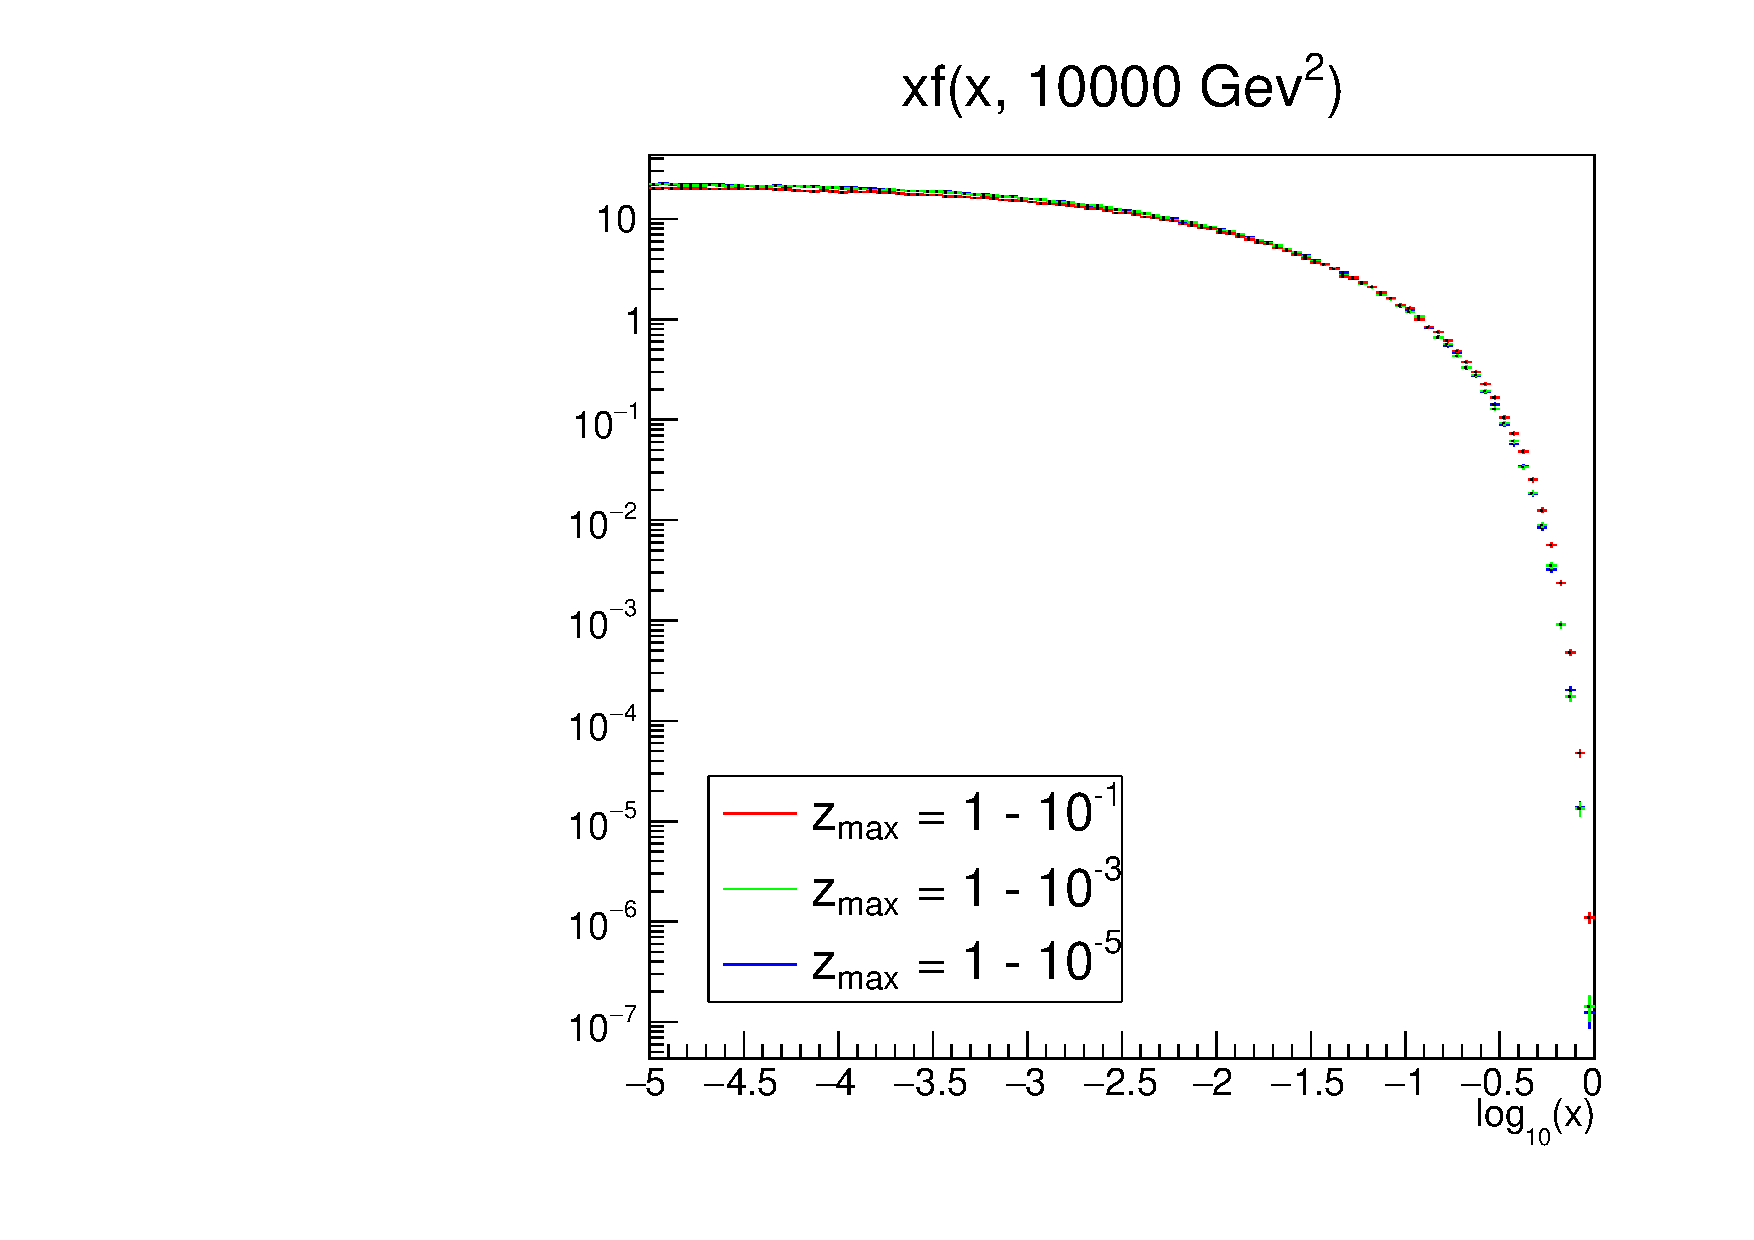
\includegraphics[width=\linewidth]{d-gg_density_mms.pdf}
			\caption{momentum weighted density}
			\label{fig:simp_3}
    \end{subfigure}
      \hspace{20pt}
    \begin{subfigure}[b]{0.45\linewidth}
      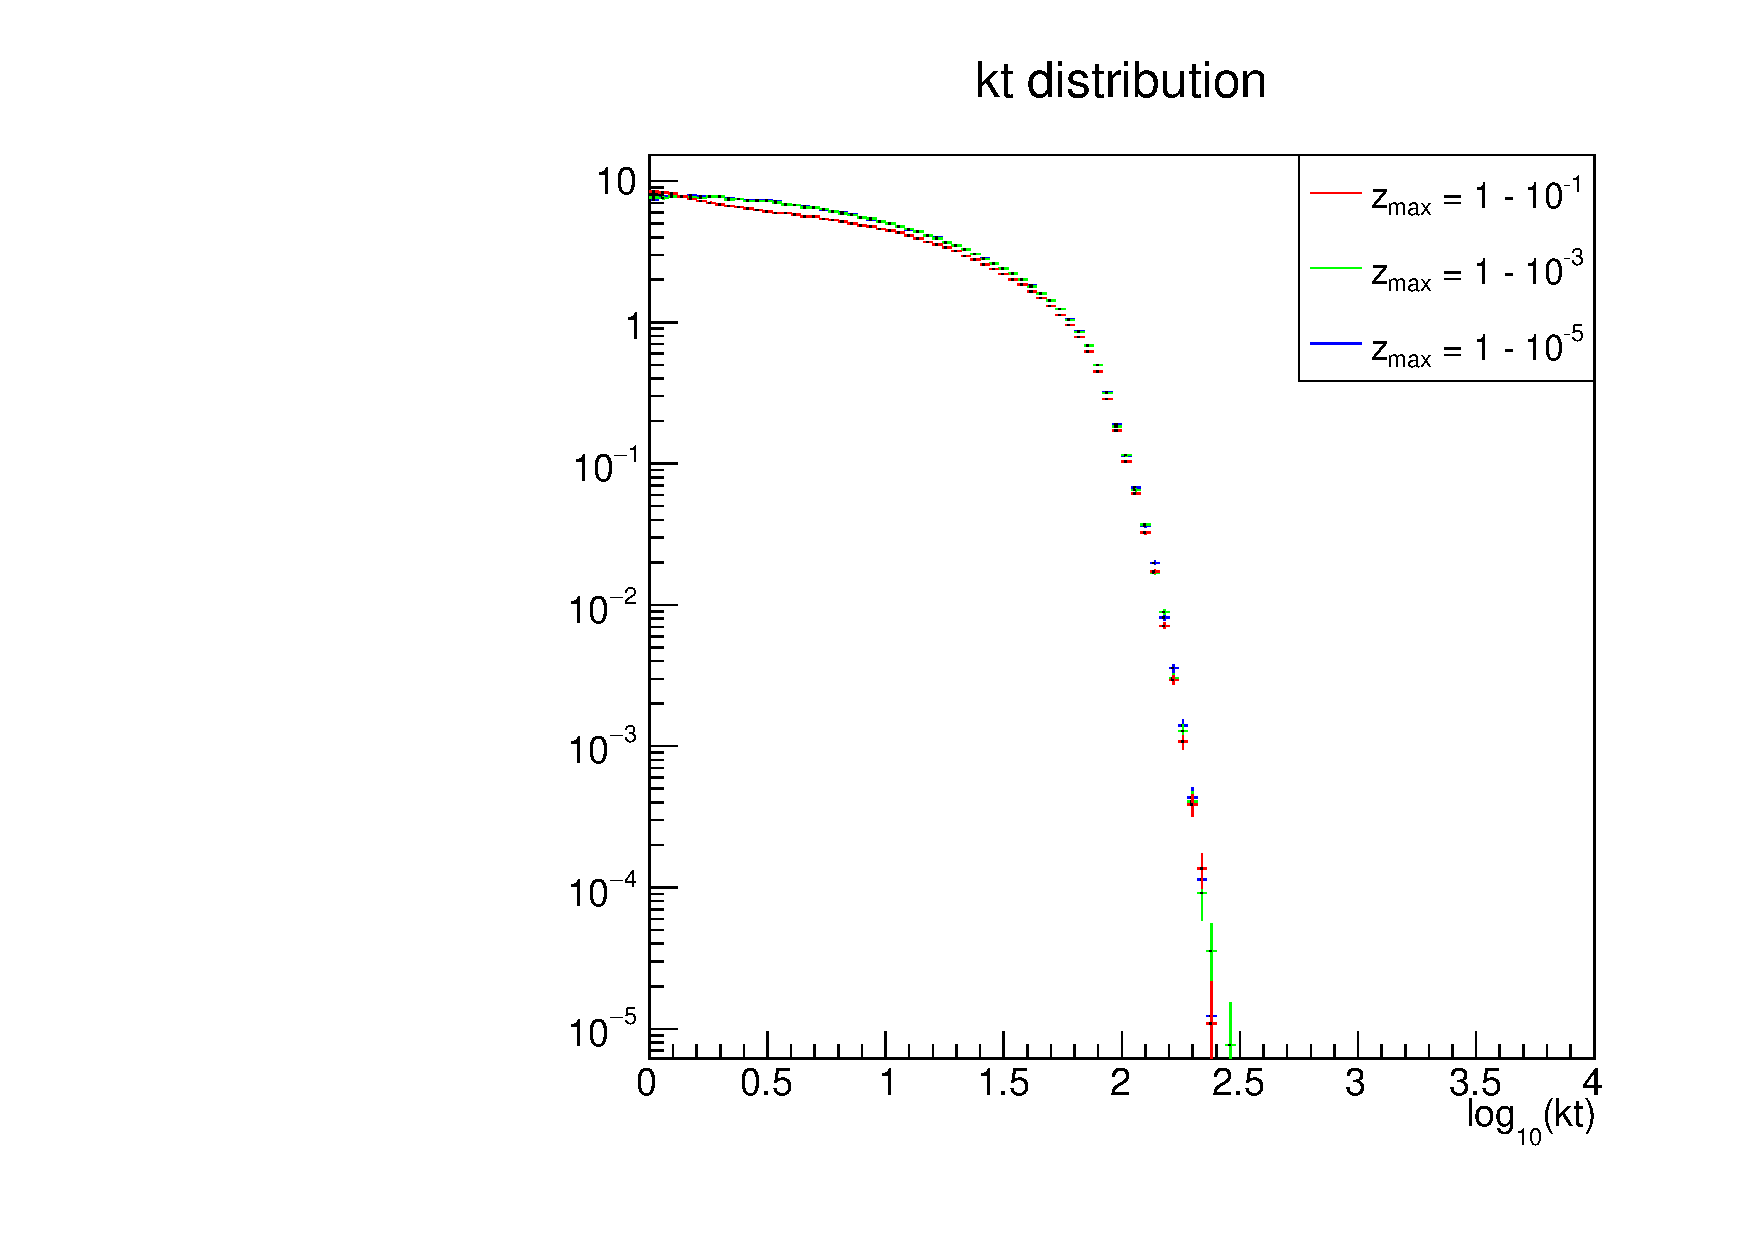
\includegraphics[width=\linewidth]{d-gg_kt_mms.pdf}
			\caption{transverse momentum distribution}
			\label{fig:simp_3}
    \end{subfigure}
    \caption{Evolved gluon densities, fixed $z_{min}$, variable $z_{max}$.}
		\label{fig:simp_3}
    \end{figure*}

    We finally get stable results. We saw here that we can hope to get consistent results independently 
    of the arbitrary choice of $z_{max}$ (provided that it is reasonably close to 1). This is because 
    bringing $z_{max}$ closer to 1 increase the amount of splittings generated, but also increase the probability
    to generate the splitting variable $z_i$ closer to 1, thus making the splittings less impactful, for both
    the $x$ and the $k_t$ distribution. \\ 
    
    Now we can investigate what happens when we choose transverse ordering (see \equref{eq:simp_trord}) for 
    the $k_t$ generation. It doesn't affect the $x$ density, but it should of course change the $k_t$ densities. 
    Firstly, here is an example of gluon event generation, with $z_{min} = 0.1$ and $ z_{max} = 0.9$ : 

    \begin{figure*}[h]
    \centering
    \begin{subfigure}[b]{0.37\linewidth}
      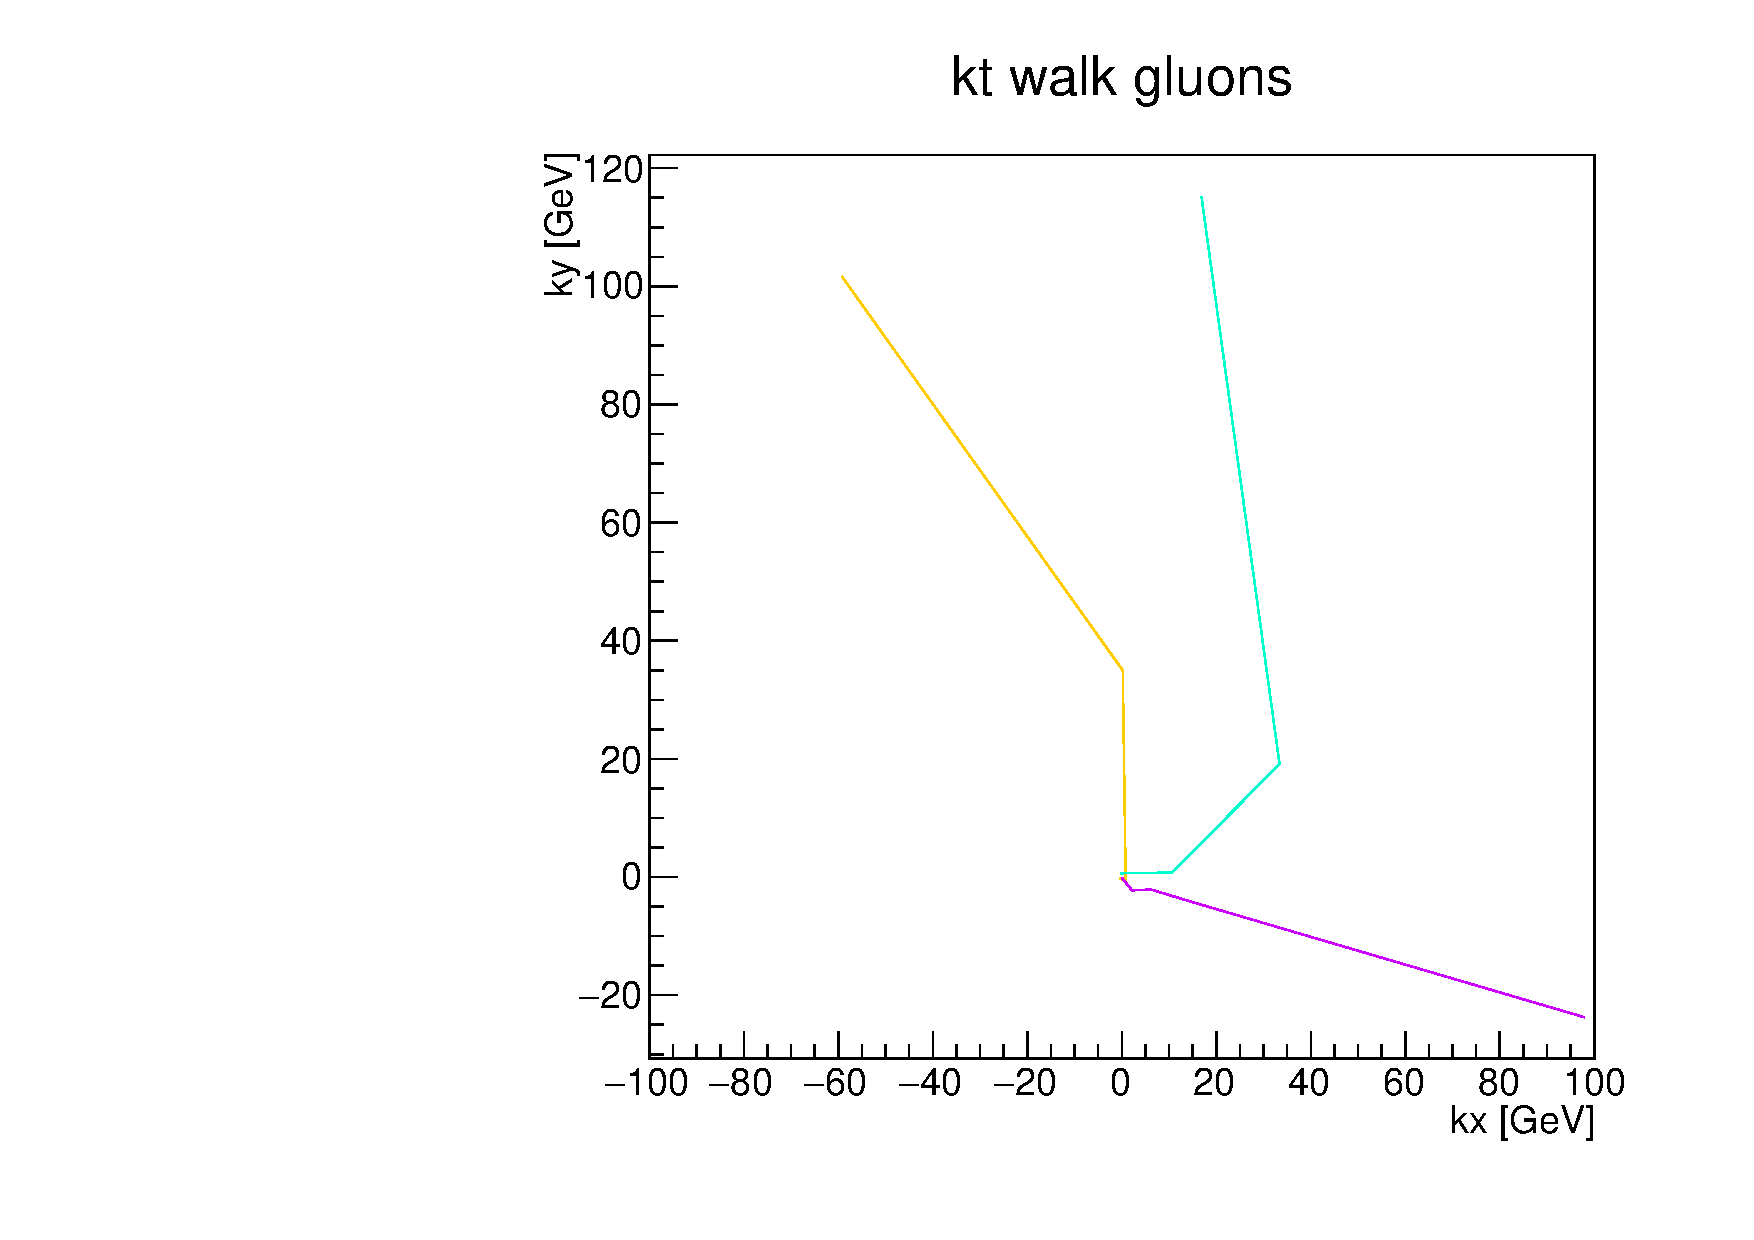
\includegraphics[width=\linewidth]{a-to-walksktxy-Pgg.pdf}
			\caption{sample gluon $k_t$ generation}
			\label{fig:simp_egz1}
    \end{subfigure}
      \hspace{20pt}
    \begin{subfigure}[b]{0.37\linewidth}
      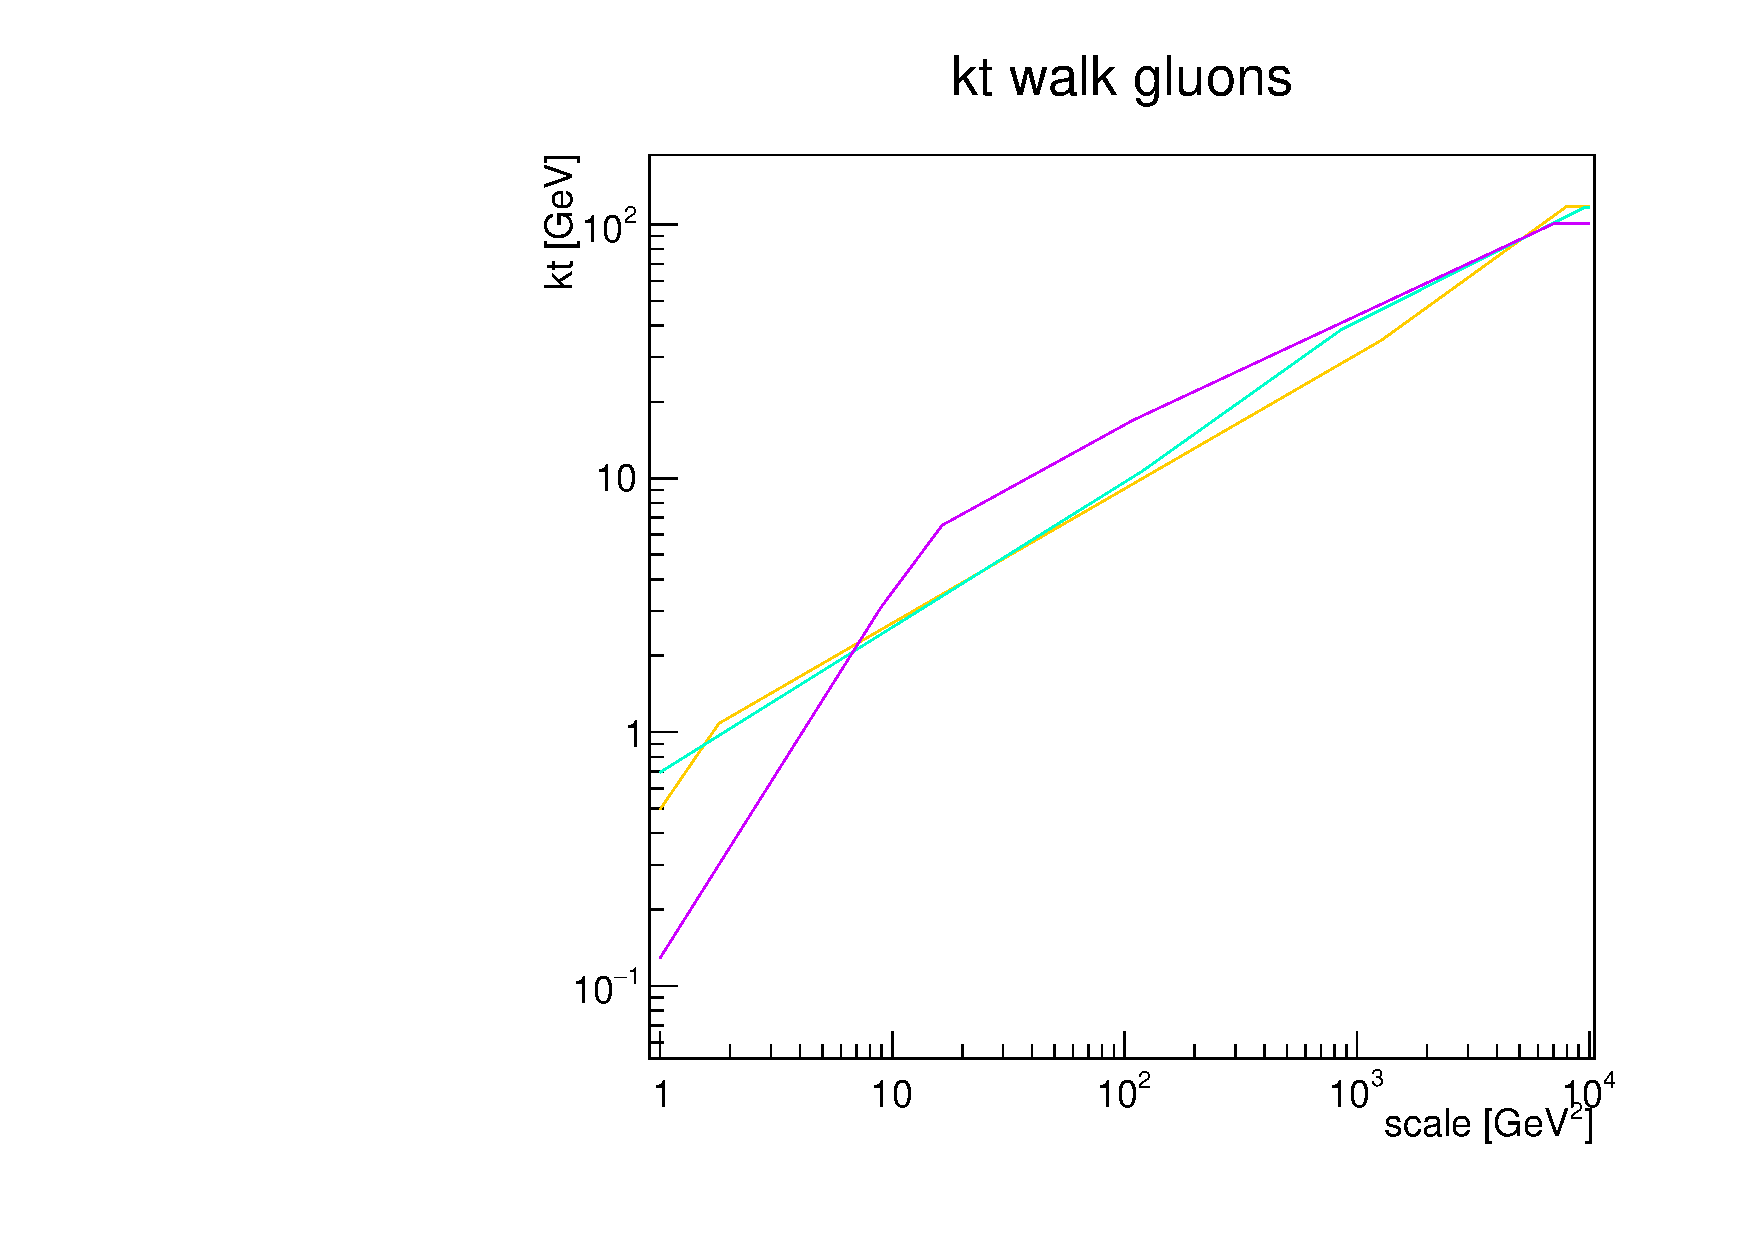
\includegraphics[width=\linewidth]{a-to-walkskt-Pgg.pdf}
			\caption{sample gluon $k_t$ evolution}
			\label{fig:simp_egkxy1}
    \end{subfigure}
    \caption{$k_t$ evolution with transverse ordering, for a sample of three gluons, $z_{max} = 0.9$.}
		\label{fig:simp_eg1}
    \end{figure*}

    \vfill\eject
    Now successive steps always do a larger $k_t$ jump. But we can already anticipate an issue here. 
    The amount of splitting is sensitive to $z_{max}$, and so is the $z_i$ generation, but the $k_t$ generation
    is only sensitive to the former, since \equref{eq:simp_trord} does not depend on $z_i$. We can 
    expect to lose $z_{max}$ independence, and this is indeed the case : 

    \begin{figure*}[h]
    \centering
    \begin{subfigure}[b]{0.45\linewidth}
      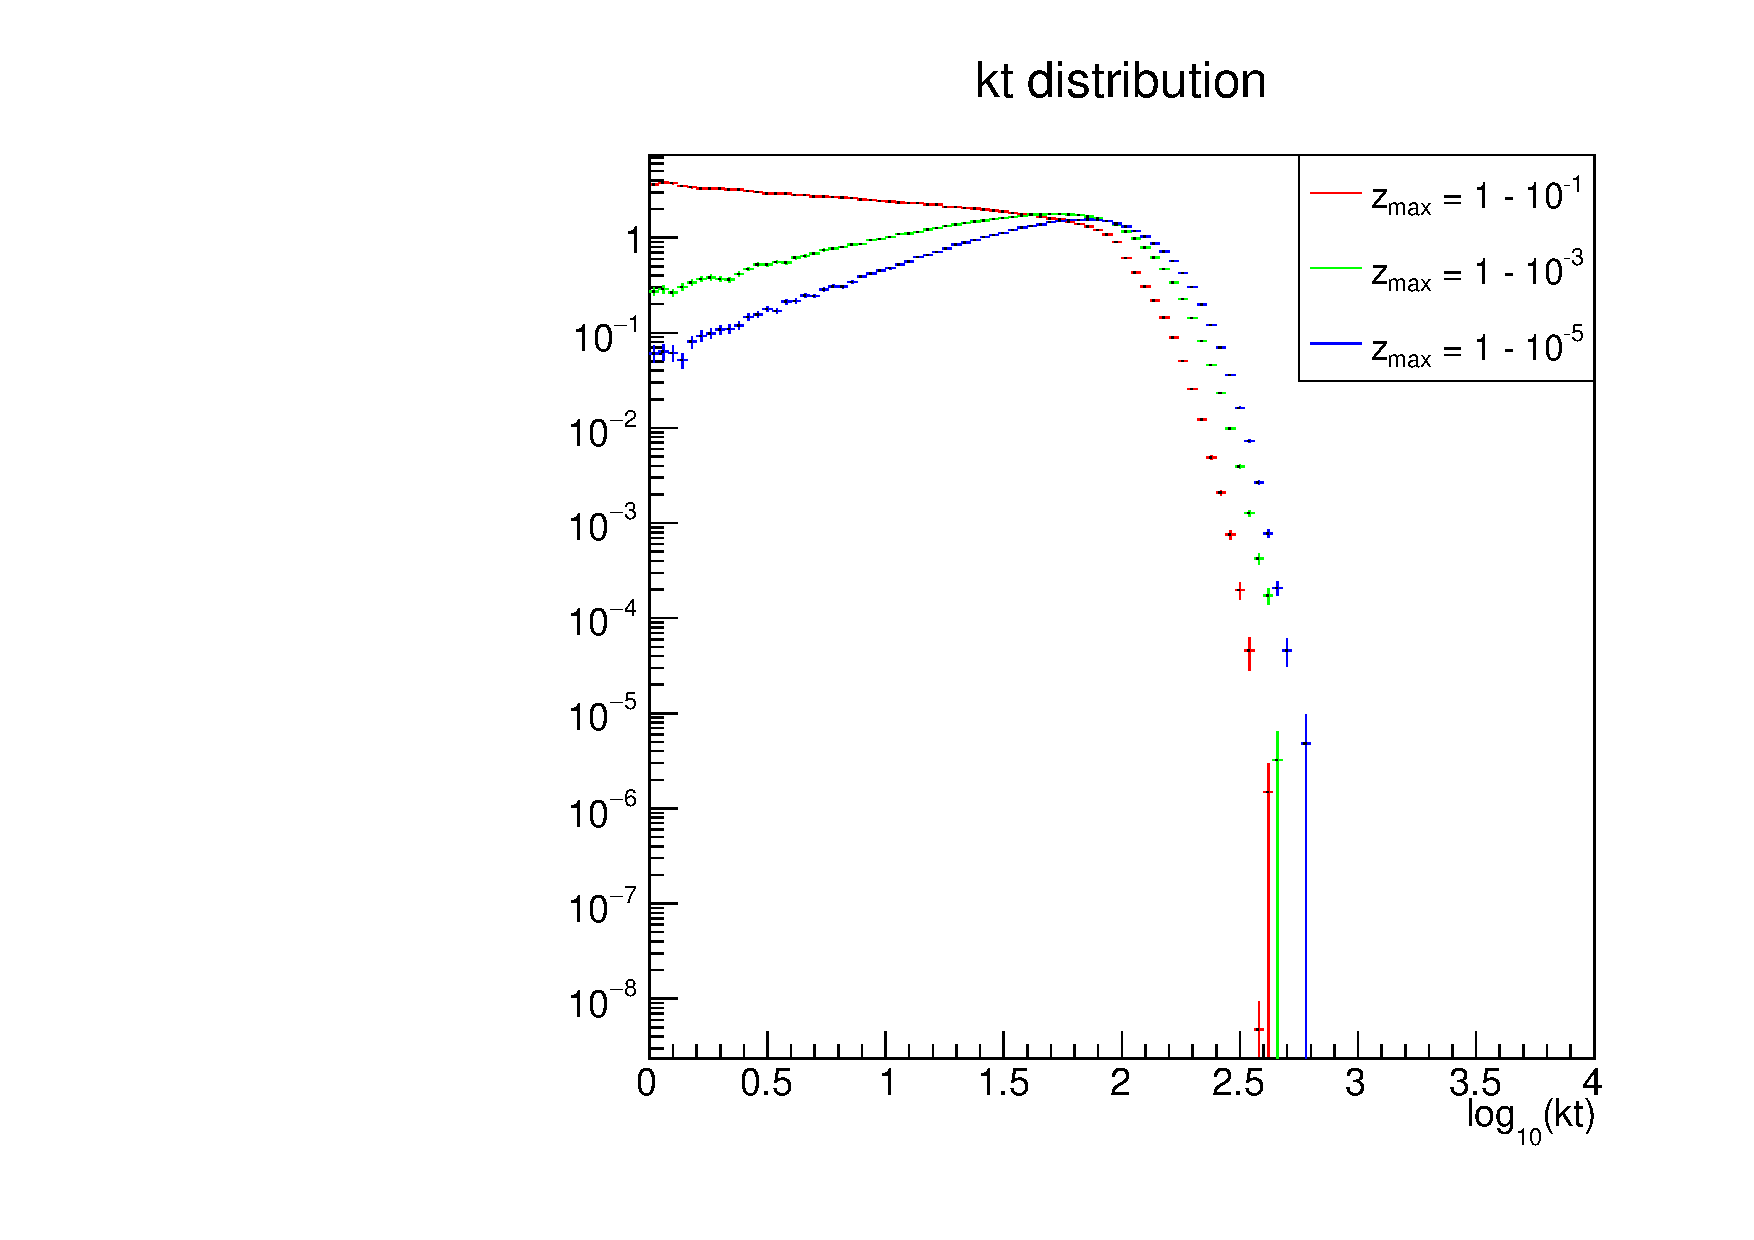
\includegraphics[width=\linewidth]{to-gg_kt_mms.pdf}
			\caption{gluon distribution}
			\label{fig:simp_kt2g}
    \end{subfigure}
      \hspace{20pt}
    \begin{subfigure}[b]{0.45\linewidth}
      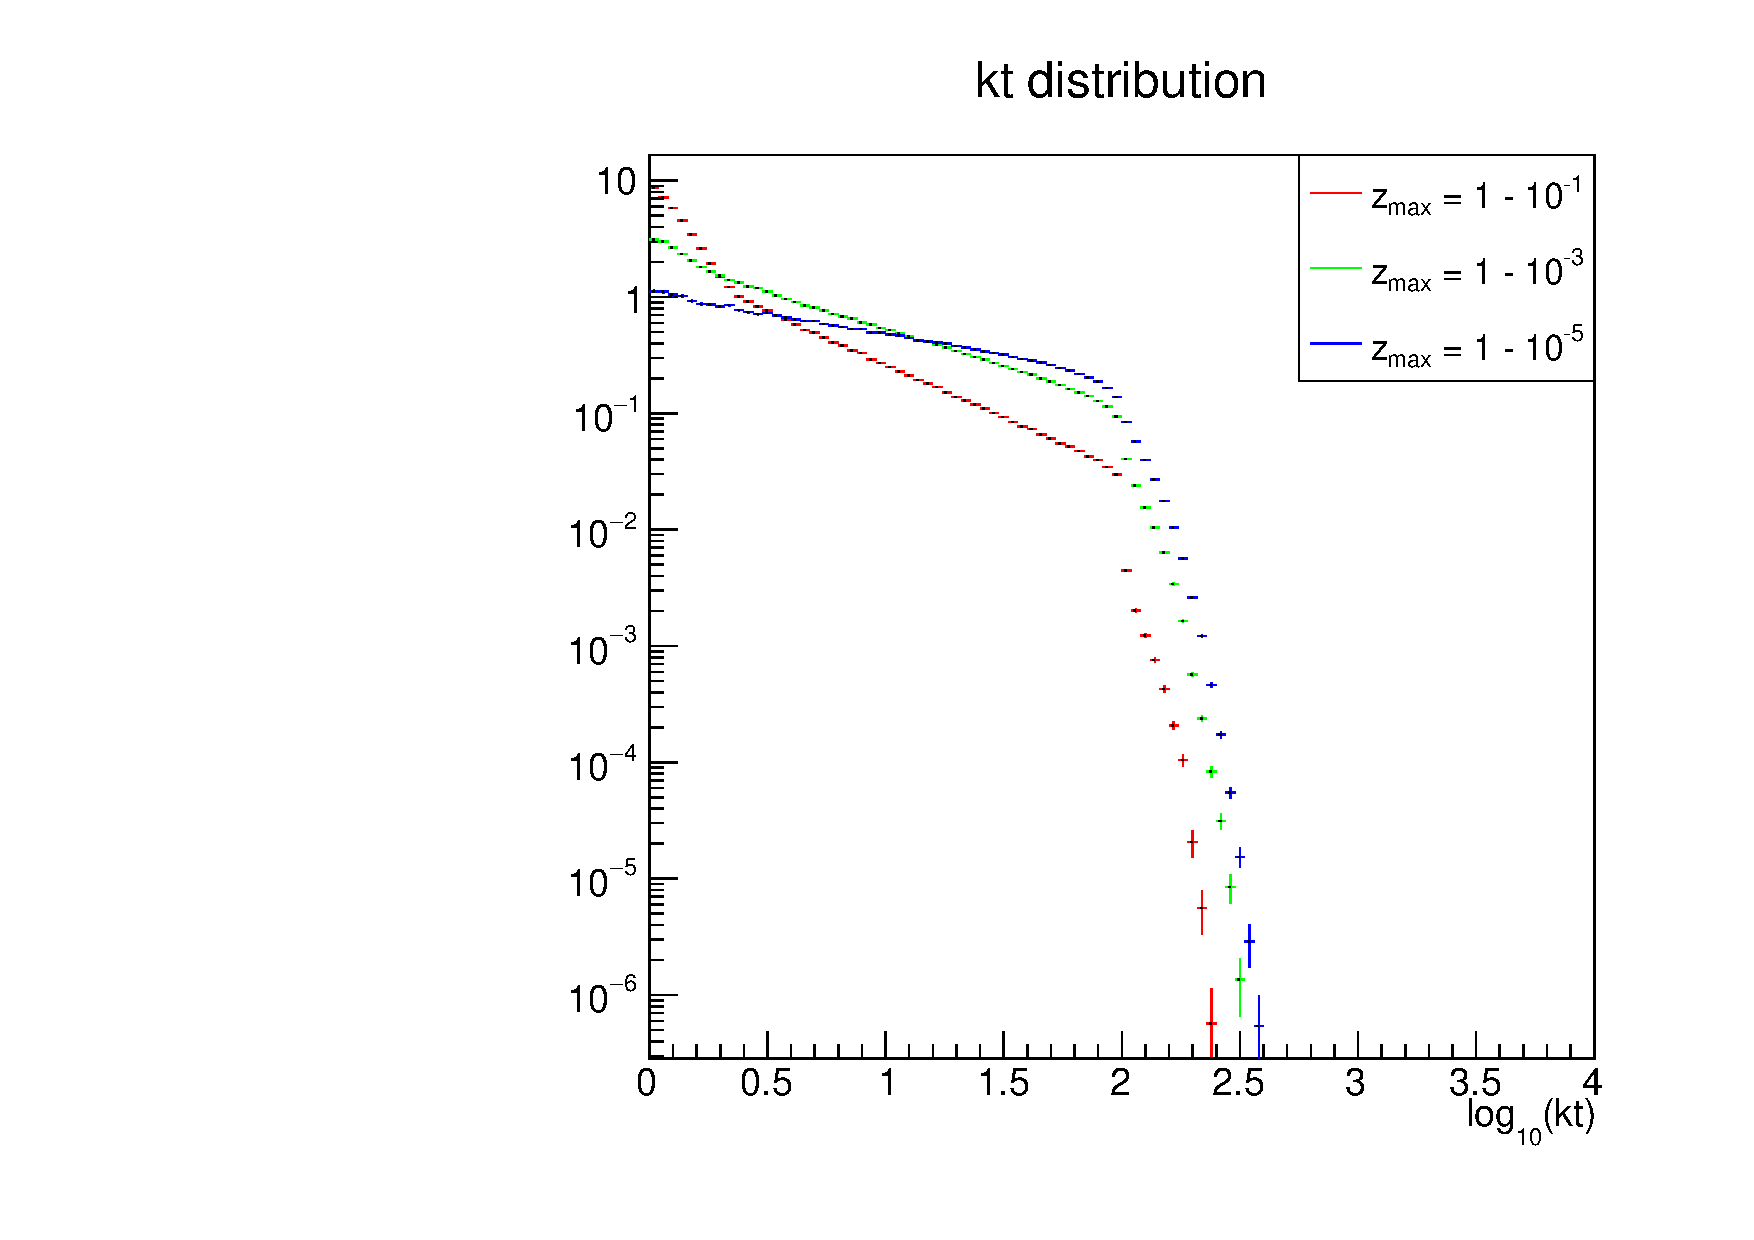
\includegraphics[width=\linewidth]{to-qq_kt_mms.pdf}
			\caption{quark distribution}
			\label{fig:simp_kt2q}
    \end{subfigure}
    \caption{Evolved $k_t$ distribution, transverse ordering, variable $z_{max}$}
		\label{fig:simp_kt2}
    \end{figure*}

    Angular ordering is a better choice, because it correctly compensates its 
    sensitivity to the amount of splittings with its $z_i$ dependence. We will 
    see in the next chapter the physical explanation for this.\\

    Comparer avec des distributions initiales réalistes ?
    

    \section{Summary and perspectives}

    Résumer les étapes, expliquer ce qui changera dans l'application complète.
    Rôles différents de $z_{min}$ et $z_{max}$, trouver une 
    bonne justification pour la valeur de $z_{min}$.



\newpage

\chapter{À déterminer}
Développement des formules utilisées dans le code, \cite{Hautmann_2018}

\newpage

\chapter{À déterminer+}
Fonctionnement du code...

\newpage

\chapter*{Conclusion}
\addcontentsline{toc}{chapter}{Conclusion}

\newpage

\chapter*{Annexes}
\addcontentsline{toc}{chapter}{Annexes}
\section*{Annex A}
\addcontentsline{toc}{section}{Annex A}


\newpage

\section*{IA use}

\printbibheading[heading=bibintoc]
\printbibliography[heading=subbibintoc, keyword={sourcebook}, title={Textbooks and lecture notes}]
\printbibliography[heading=subbibintoc, keyword={thesis}, title={Thesis}]
\printbibliography[heading=subbibintoc, keyword={article}, title={Articles}]

\end{document}